\chapter{Design} \label{Design}

 \todo*{15-20\%; explains complete processing chain; explains what methods are used; for someone that wants to know what was done in detail}

Based on the findings in chapter \fullref{Background} and extended with use-cases the requirements for the framework are specified in \fullref{Requirements}. In \fullref{Decentralized, Distributed Computing} specific requirements in context of complex processes are substantiated with algorithms for decentralized, distributed computing. Finally, a draft design is presented in \fullref{Architecture}.

	\section{Requirements} \label{Requirements}
	
	In general this thesis follows the FURPS+ system for requirements as described by \textcite{Online:FURPS}: 
	requirements are categorized into functional and non-functional requirements:
	\begin{alignat*}{1}
		& \begin{rcases*}
			\mathmakebox[\widthof{\text{Supportability}}][l]{\text{Functionality}} & \quad
			\end{rcases*} \mathmakebox[\widthof{\text{non-functional requirements}}][l]{\text{functional requirements}} \\
		& \begin{rcases*}
			\text{Usability} & \quad \\
			\text{Reliability} & \quad \\
			\text{Performance} & \quad \\
			\text{Supportability} & \quad
		\end{rcases*} \text{non-functional requirements}
	\end{alignat*}
	
	The functional and non-functional requirements are specified in \ref{Functional Requirements} and \ref{Non-Functional Requirements}. 
	
	\subsection{Functional Requirements} \label{Functional Requirements}
	
	Functional requirements define the functions the framework has to offer to meet the acceptance criteria. Based on chapter \fullref{Background} we can divide the requirements into two main fields: features regarding the accurate computation of the \gls{SMPC} protocols and functions required to compensate the lack of a \gls{MANET} \gls{API} and technical limitations.
	Figure \ref{figure:requirements use-case node} presents the general functionality a party - respectively a node - expects from the system: especially the need for a secure channel and the limitation to run the \gls{SMPC} only with nearby computation partners is caused by the missing multi-hop capabilities.
	
	\begin{figure}[!htb] % h for placement here
	\caption{\gls{UML} use-case diagram for the general functional requirements of a node} \label{figure:requirements use-case node}
	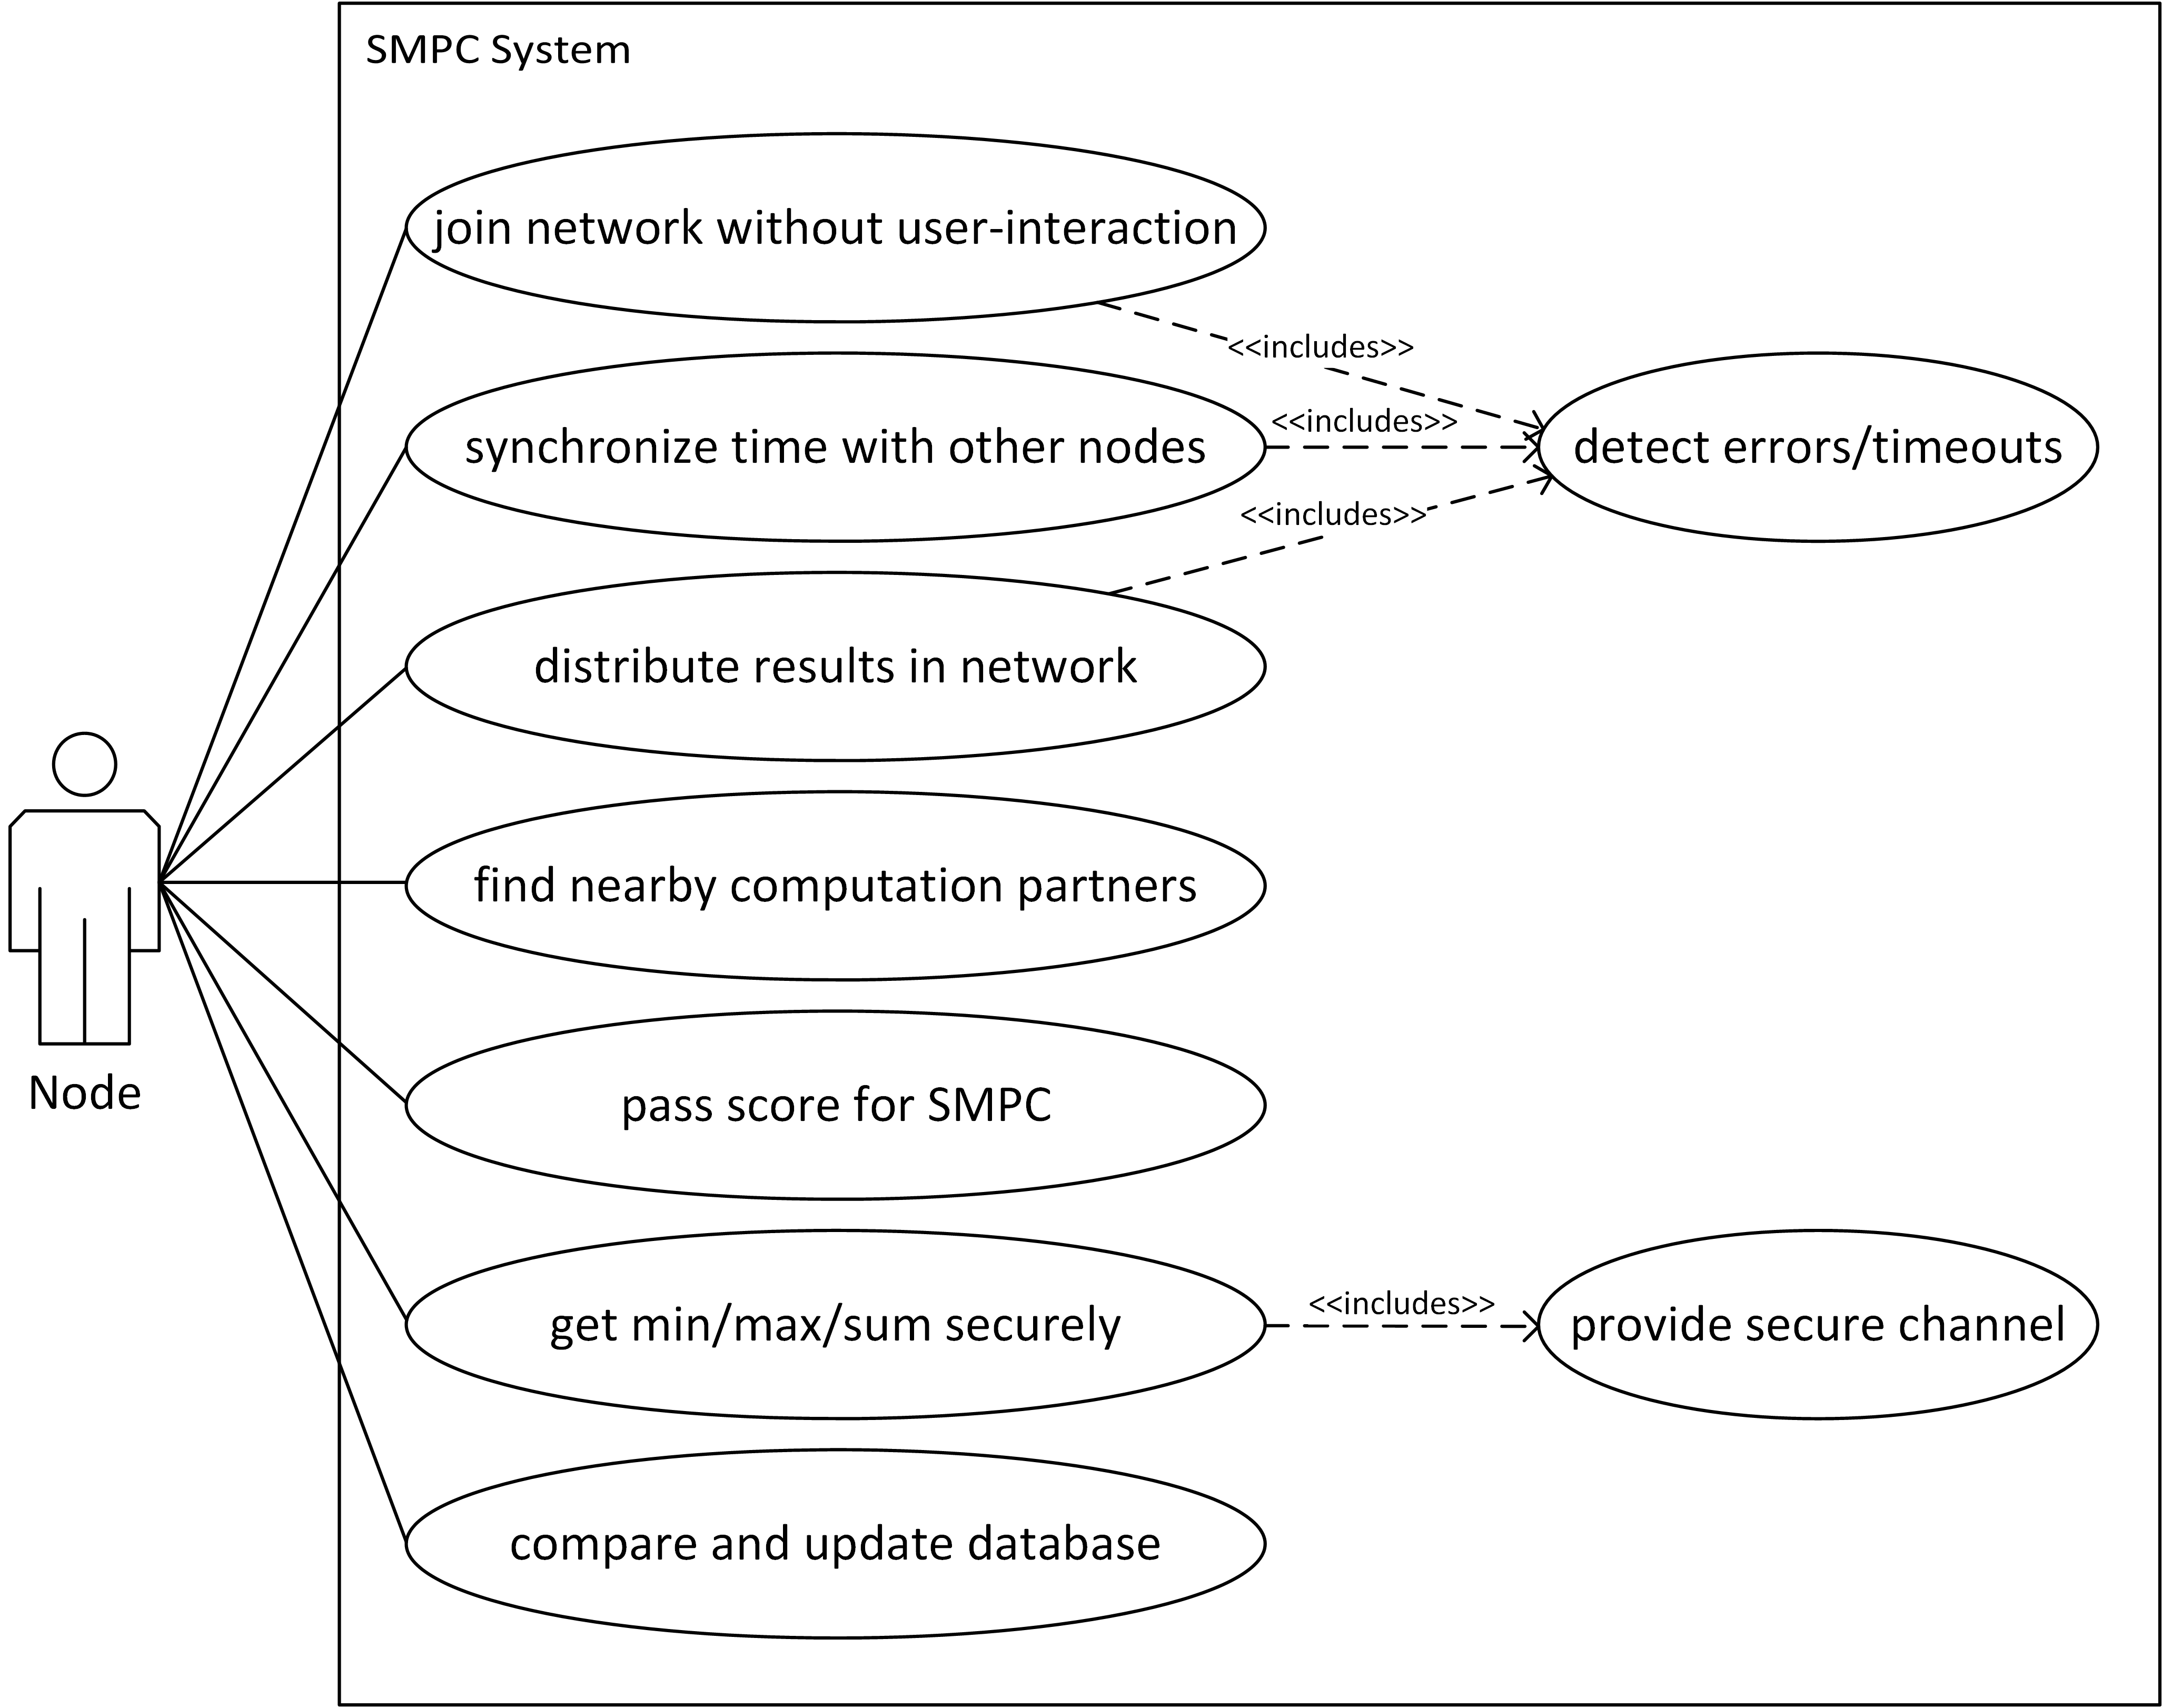
\includegraphics[scale=0.85]{figures/use-case-node.png}
	\end{figure}

	Since most functions (like the time synchronization and the multi-party computation) require the interaction between nodes, these processes need to be coordinated. In a distributed system there is no central authority, so a node has to become the temporal leader or coordinator for the duration of a process. In figure \ref{figure:requirements use-case coordinator} the processes requiring coordination are described as use-cases from the view of a temporal coordinator.
	
	\begin{figure}[!htb] % h for placement here
	\caption{\gls{UML} use-case diagram for the functional requirements for the coordinator} \label{figure:requirements use-case coordinator}
	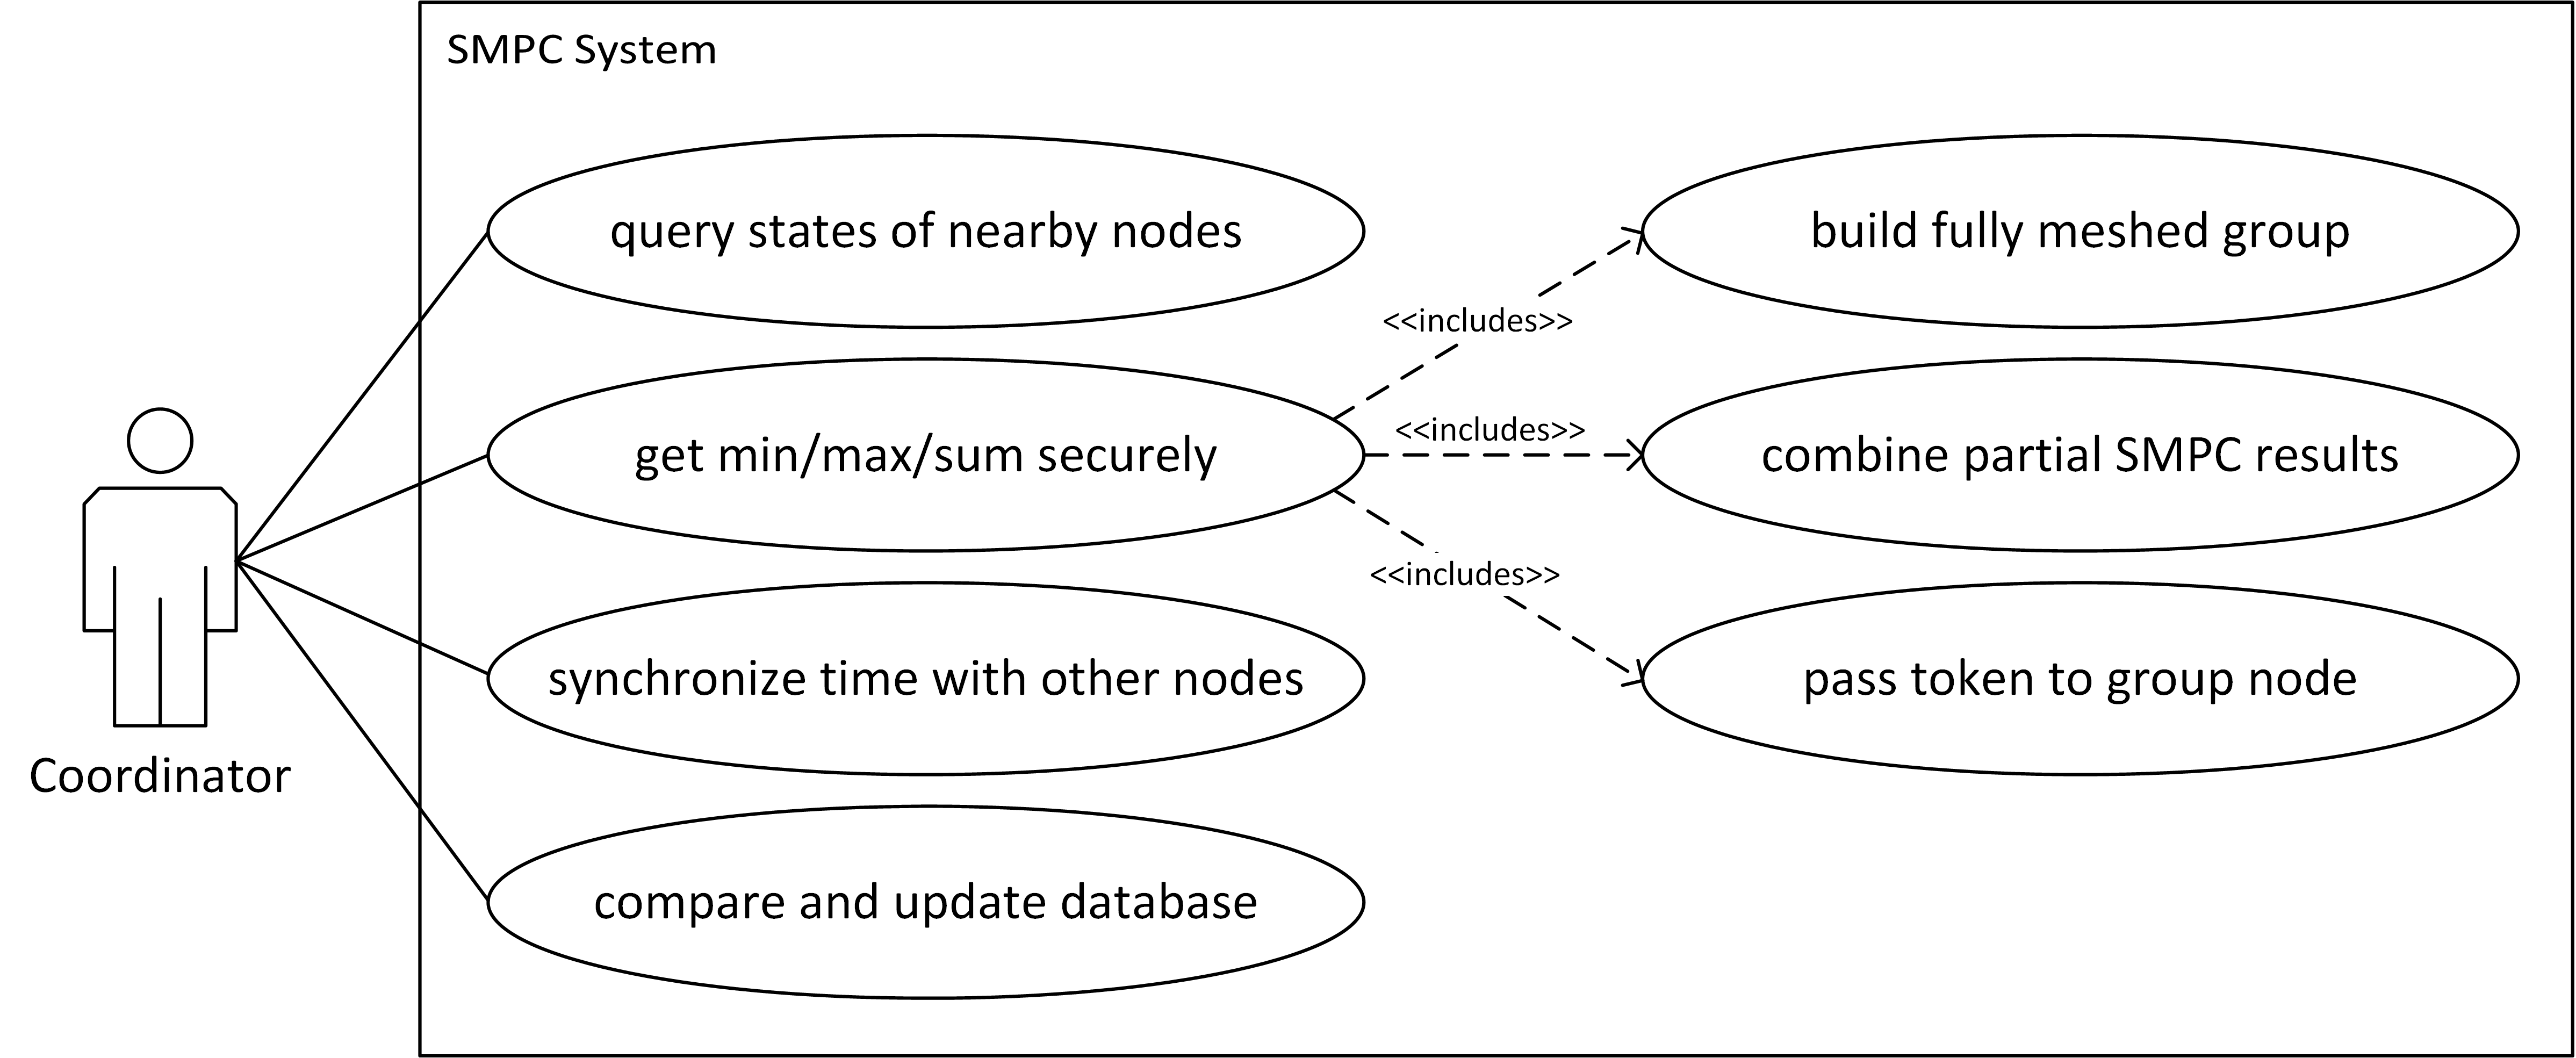
\includegraphics[scale=0.75]{figures/use-case-coordinator.png}
	\end{figure}

	Based on the use-cases functional requirements can easily be identified and specified. In table \ref{table:functional requirements} the functional requirements are stated as user-stories, alongside assumptions and targeted tests.


	\begin{table}[!htb] % h for placement here
		\centering
		\caption{Functional requirements} \label{table:functional requirements}
		\begin{tabular}{|l|p{\textwidth*4/5}|}
			\toprule
			Name & \funcreq{Pairing-less Connection}\label{req:Pairing-less Connection} \\ \midrule
			Requirement & As a node I want to join the system without having to pair with other devices so that the system remains unobtrusive. \\
			Assumptions & Device has Bluetooth capabilities with \gls{RFCOMM} protocol. \\ \midrule
			Name & \funcreq{Heartbeat}\label{req:Heartbeat} \\ \midrule
			Requirement & As a node I need to inform my coordinator if my computation is running longer than expected so that the system does not assume that the process has failed. As a coordinator I need to inform all group nodes if a computation is running longer than expected. \\
			Assumptions & Hosting system provides system time. \\ \midrule
			Name & \funcreq{Non-termination Detection}\label{req:Non-termination Detection} \\ \midrule
			Requirement & As a node I must be able to detect a communication problem so that I can reset my status. \\
			Assumptions & Hosting system provides system time. \\ \midrule
			Name & \funcreq{Coordinator Election}\label{req:Coordinator Election} \\ \midrule
			Requirement & As a node I want to become coordinator for nearby nodes so that communication can be organized. \\ \midrule
			Name & \funcreq{Token-Passing}\label{req:Token-Passing} \\ \midrule
			Requirement & As coordinator I want to be able to assign a group-member to coordinate a subprocess so that direct communication between group-members can be established. \\ \midrule
			Name & \funcreq{Secure Multi-Party Computation Module}\label{req:SMPC Module} \\ \midrule
			Requirement & As a coordinator I want to form a group of fully meshed nodes and coordinate the execution of the secure addition and secure comparison protocols using a secure communication channel. \\ \todo*{visualize finding fully-meshed nearby group in mesh network}
			Assumptions & Group size $>2$. All group-members are time-synchronized and have a score within the same time-frame limits. \\
			Testability & Unit tests to proof correctness of implementation. Performance-tests with different number of computation partners and validation of result. \\ \midrule
			Name & \funcreq{Clock Synchronization}\label{req:Clock Synchronization} \\ \midrule
			Requirement & As coordinator I want to synchronize the clocks of nearby nodes so that computation results are not biased because of different time settings. \\
			Testability & Unit tests to proof correctness of implementation. \\ \midrule
			Name & \funcreq{Database Synchronization}\label{req:Database Synchronization} \\ \midrule
			Requirement & As coordinator I want to compare my database status with nearby nodes without having to compare entry-wise and exchange entries. \\
			Assumptions & Participating nodes are idle and not waiting for a computation.\\
			\bottomrule
		\end{tabular}
	\end{table}

	\FloatBarrier
	\subsection{Non-Functional Requirements} \label{Non-Functional Requirements}

	Non-functional requirements describe quality attributes the system has to comply to. Two use-cases from a developer view are illustrated in figure \ref{figure:requirements use case developer}.

	\begin{figure}[!htb] % h for placement here
	\caption{\gls{UML} use case diagram for developer} \label{figure:requirements use case developer}
	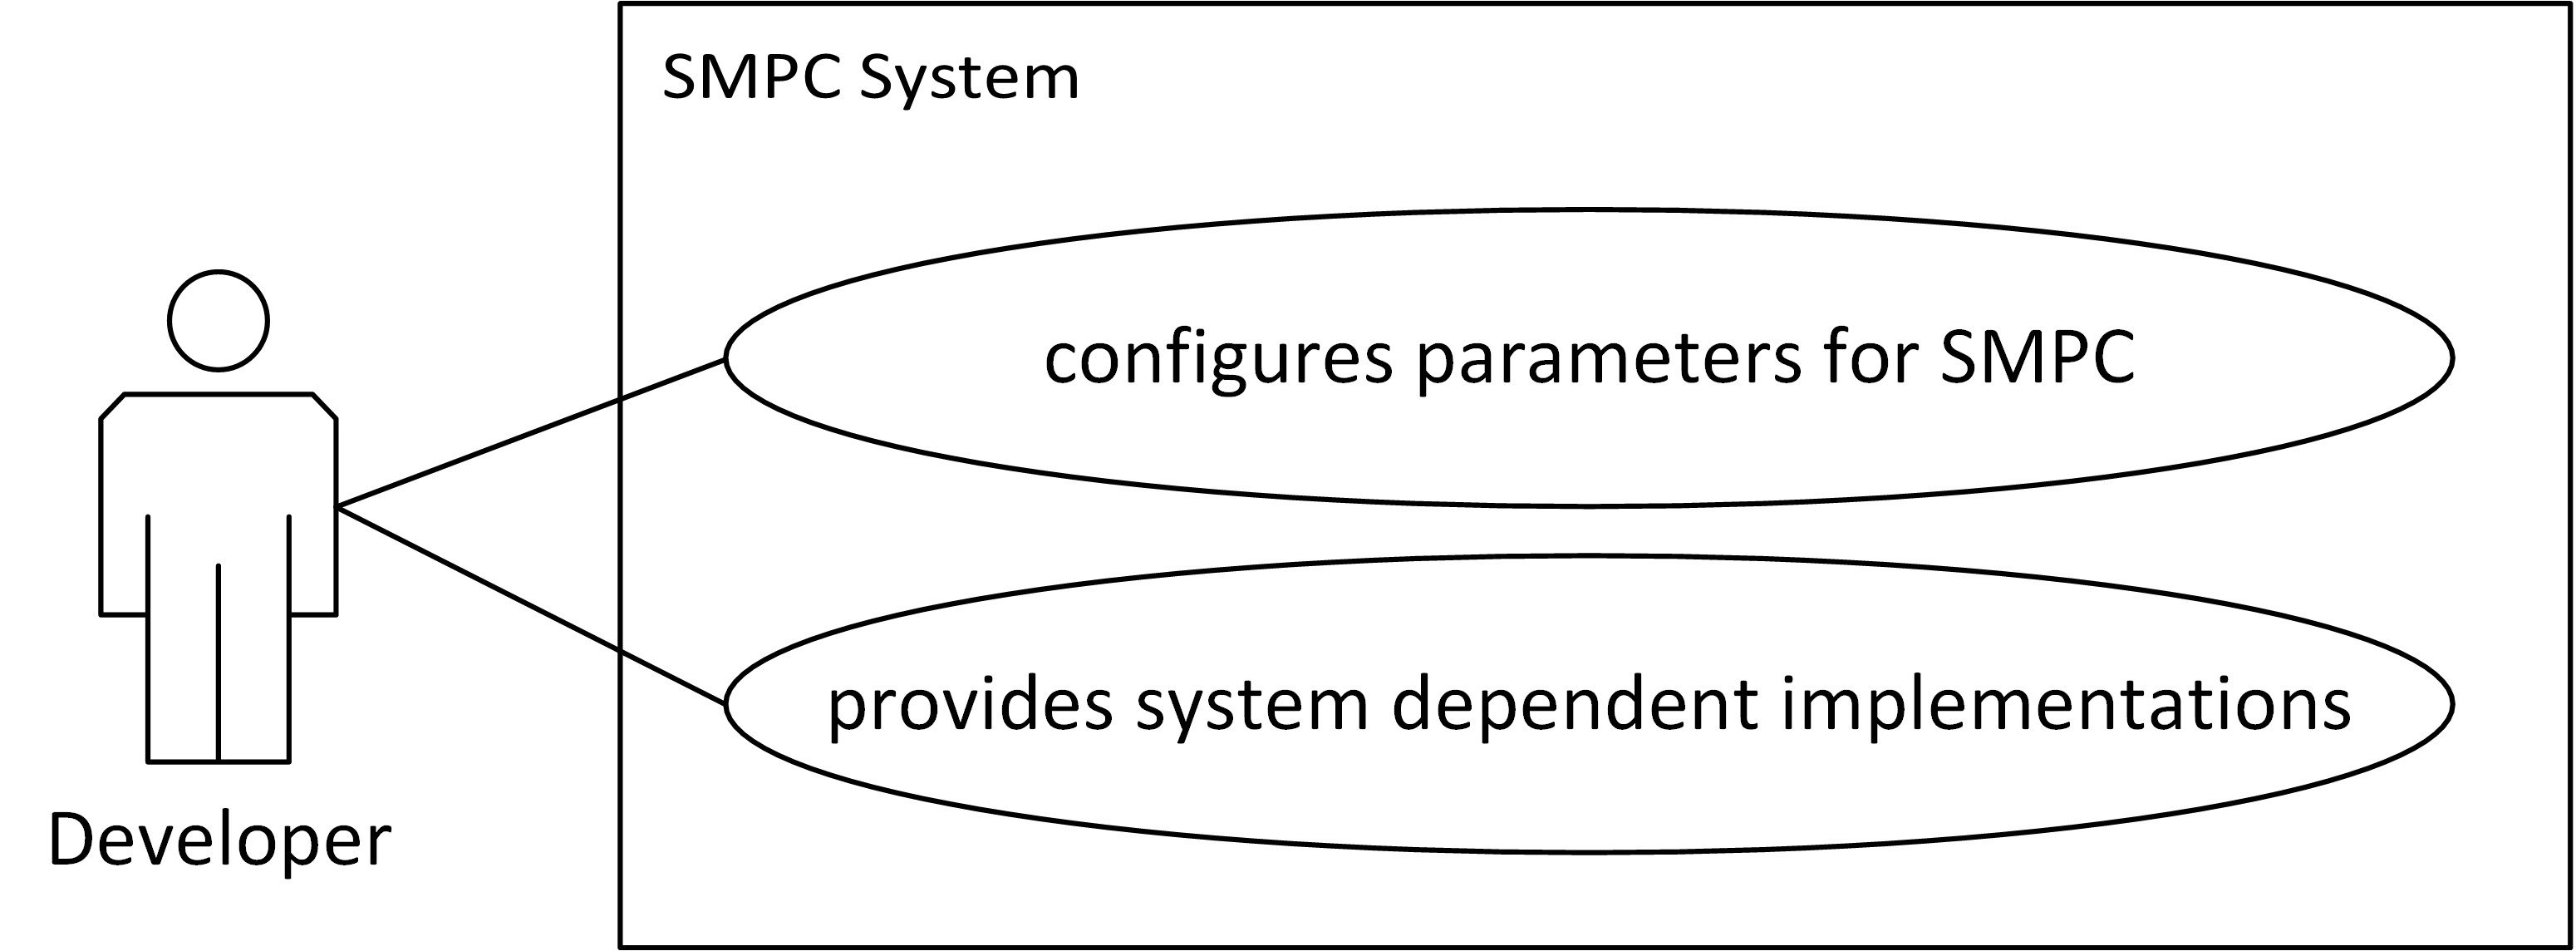
\includegraphics[scale=0.85]{figures/use-case-developer.png}
	\end{figure}

	Based on the use-cases for developers and general demands regarding the maintainability, expandability and performance to make the framework applicable for real-life settings non-functional requirements can be specified as listed in table \ref{table:non-functional requirements}.

	\begin{table}[!htb] % h for placement here
		\centering
		\caption{Non-functional requirements} \label{table:non-functional requirements}
		\begin{tabular}{|l|p{\textwidth*4/5}|}
			\toprule
		Name & \nonfuncreq{Usability}\label{req:Usability} \\ \midrule
		Requirement & The framework shall be configurable, so that a developer using the framework can configure the settings for the \gls{SMPC}. \\ \midrule
		Name & \nonfuncreq{Maintainability}\label{req:Supportability} \\ \midrule
		Requirement & The framework shall be maintainable, so that the code and documentation make it clear for a developer what callbacks have to be implemented and how the framework can be used in an Android device. \\ \midrule
		Name & \nonfuncreq{Performance}\label{req:Performance} \\ \midrule
		Requirement & The framework shall be secure while providing enough performance, that computations can properly terminate for nodes that move at walking speed ($\approx1\frac{m}{s}$). \\ \midrule
		Name & \nonfuncreq{Expandability}\label{req:Expandability} \\ \midrule
		Requirement & The frameworks coupling with the wireless technology shall be loosely, so that the system can be extended without having to touch core functionalities regarding the \gls{SMPC}.  \\ \bottomrule
		\end{tabular}
	\end{table}
		
	\FloatBarrier
	
	\section{Decentralized, Distributed Computing} \label{Decentralized, Distributed Computing}
	
		While the protocols for secure addition and secure comparison and thereby the requirement \ref{req:SMPC Module} are already well-defined (compare \ref{Secret Sharing}, \ref{Secure Addition Protocol} and \ref{Secure Comparison Protocol}) other functional requirements need further methodical substantiation. \ref{req:Coordinator Election} and \ref{req:Token-Passing} are addressed in \ref{Coordinator Election}, \ref{req:Heartbeat} and \ref{req:Non-termination Detection} are discussed in \ref{Non-termination Detection}, an algorithm for \ref{req:Clock Synchronization} is provided in \ref{Clock synchronization} and finally \ref{req:Database Synchronization} is covered in \ref{Distributed Database}.

		\subsection{Coordinator Election and Coordinator Role} \label{Coordinator Election}
		
		As discussed in \fullref{Implementability} fully featured \glspl{MANET} are currently not provided and mapping it completely in the application layer is beyond the scope of this thesis. Overcoming the technical limitation, the system can be build with sequential communications instead of parallel. As stated in \fullref{Network Topologies} communication in context of \gls{SMPC} computations is only done in a fully meshed subgroup of the network, which also simplifies the coordinator election.
		
		\noindent A node will try to become the coordinator, when \nolinebreak
		%\vspace{-\topsep}
		\begin{enumerate}
			%\itemsep-0.5em
			\item it enters the network after longer disconnection: event driven.
			\item a new personal score is ready for \gls{SMPC}: event driven.
			\item all \gls{SMPC} computations for a score are done: event driven.
			\item an event driven attempt failed and a certain amount of time passed: timer based.
		\end{enumerate}
		
		Extending requirement \ref{req:Coordinator Election} and to avoid situations of competing nodes trying to become coordinator and thereby booth repeatedly failing because neither can acquire enough computation partners, the timer based approach is supported by the exponential backoff algorithm. \textcite[p.67]{IEEE2010} describes the exponential backoff algorithm for collision detection and retransmission: if a coordinator appointment failed (equivalent to collision detection in original description) a factor for the waiting time till the next attempt is selected uniformly random from an increasing range, reducing the probability for competing coordinator candidates. The process is outlined in form of an \gls{UML} activity diagram in figure \ref{figure:coordinator exponential backoff}).
		
		\begin{figure}[htbp] % h for placement here
		\caption{\gls{UML} activity diagram for exponential backoff algorithm} \label{figure:coordinator exponential backoff}
		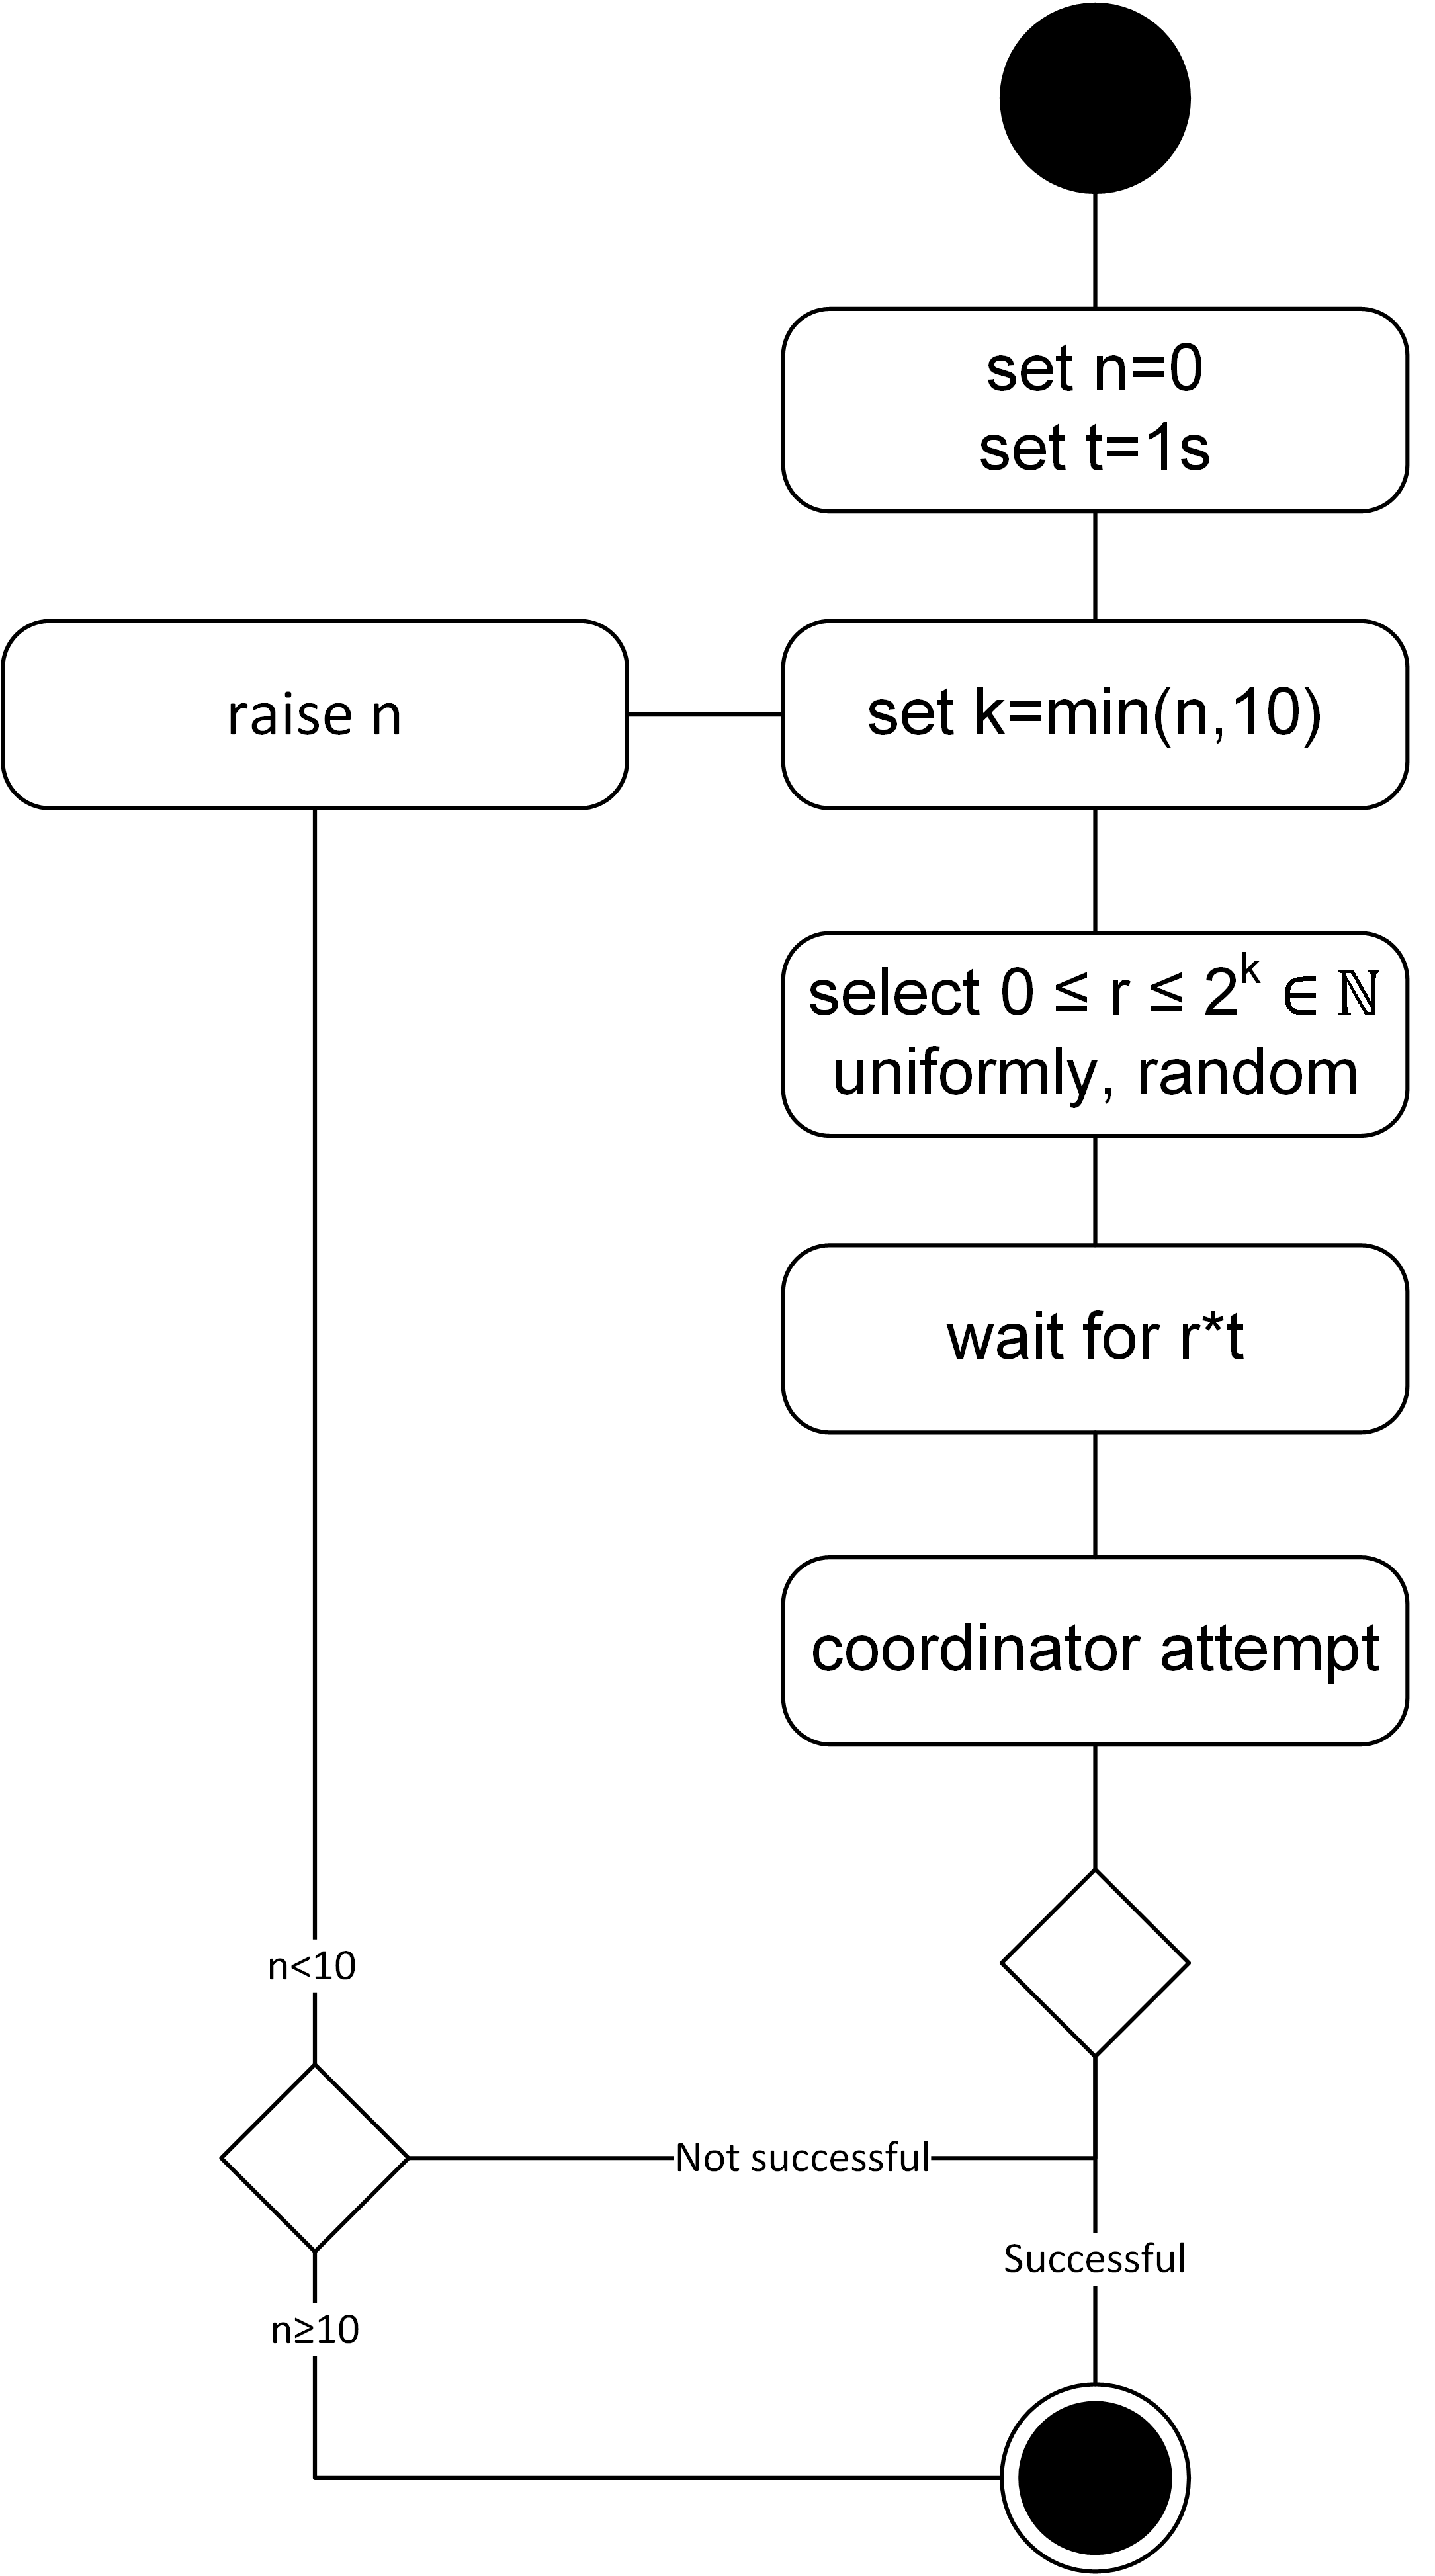
\includegraphics[scale=0.8]{figures/exponential-backoff.png}
		\end{figure}
		
		\todo*{Reduction of active connections; compare number of additional rounds needed; discuss timeouts}
		
		In regard to the execution of the \gls{SMPC} protocols in \ref{req:SMPC Module}, the coordinator has to find a computation group. In a mesh network with routing and point-to-point encryption as displayed in figure \ref{figure:Formation of fully meshed computation group - a}, the green marked coordinator can simply broadcast a computation request and responding nodes form the computation group. Caused by the technical limitations (see \ref{Implementability}), the coordinator has to find a fully meshed group within its reach. First the coordinator $n_1$ discovers nearby nodes (see figure \ref{figure:Formation of fully meshed computation group - b}). Then a list of these devices (identified by \gls{MAC} address) is sent to every neighboring node (see $n_2$ to $n_7$ in figure \ref{figure:Formation of fully meshed computation group - c}). Each node responds with the intersection of the received device list with the own list of discovered devices (see figure \ref{figure:Formation of fully meshed computation group - d}). To reduce the payload of the responses, they only contain a list of booleans, indication if the device with the same index in the received device list is seen by the device. The coordinator then computes the maximum group of fully meshed nodes and sends computation partners an associative array assigning new 8-bit ids (see figure \ref{figure:Formation of fully meshed computation group - e}), which reduce the payload in following steps. Nearby nodes, that are not part of the computation group, receive an indicator to abort the computation. Each node in the computation group has a list of the group and the assigned ids and can exchange public keys with group member, forming a fully meshed, end-to-end encrypted group (see figure \ref{figure:Formation of fully meshed computation group - f}).
		
		\begin{figure}[!htb] % h for placement here
	        \caption{Formation of fully meshed computation group} \label{figure:Formation of fully meshed computation group}
	        \centering
			\subfloat[]{%
				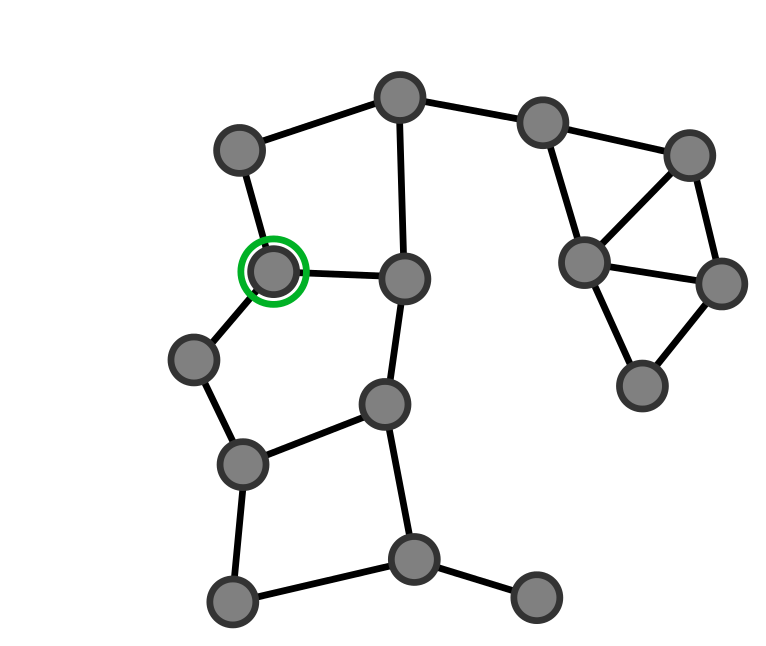
\includegraphics[scale=1.0]{figures/coordinator-1.png}
				\label{figure:Formation of fully meshed computation group - a}
			}%
			\hfill
			\subfloat[]{%
				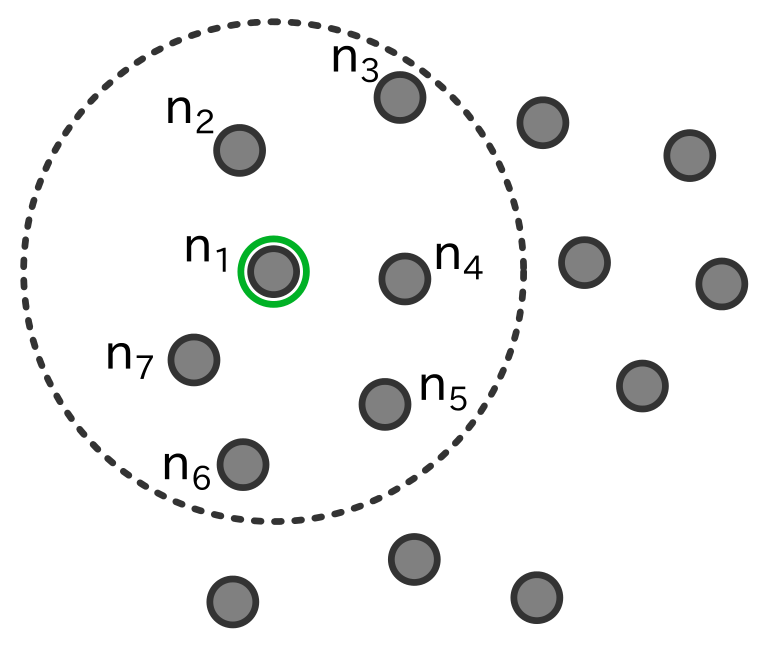
\includegraphics[scale=1.0]{figures/coordinator-2.png}
				\label{figure:Formation of fully meshed computation group - b}
			}\\
			\subfloat[]{%
				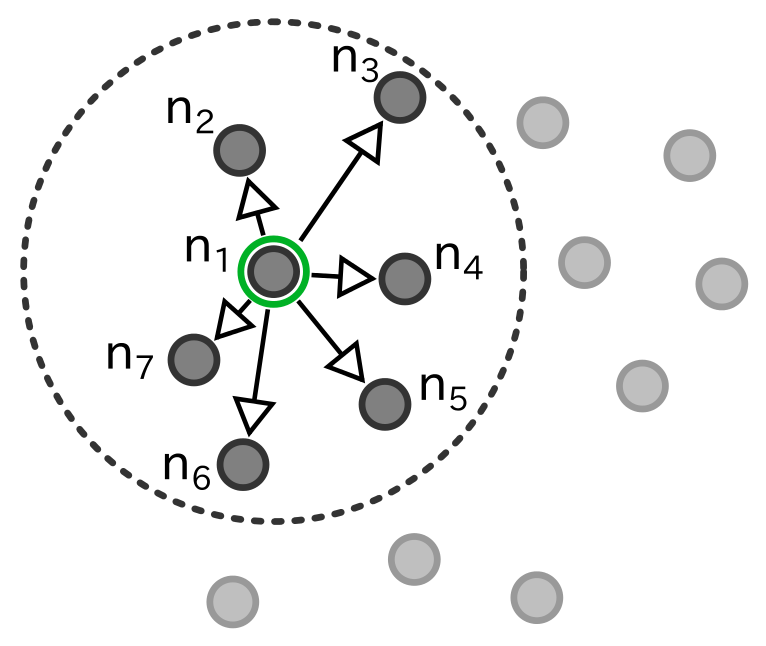
\includegraphics[scale=1.0]{figures/coordinator-3.png}
				\label{figure:Formation of fully meshed computation group - c}
			}%
			\hfill
			\subfloat[]{%
				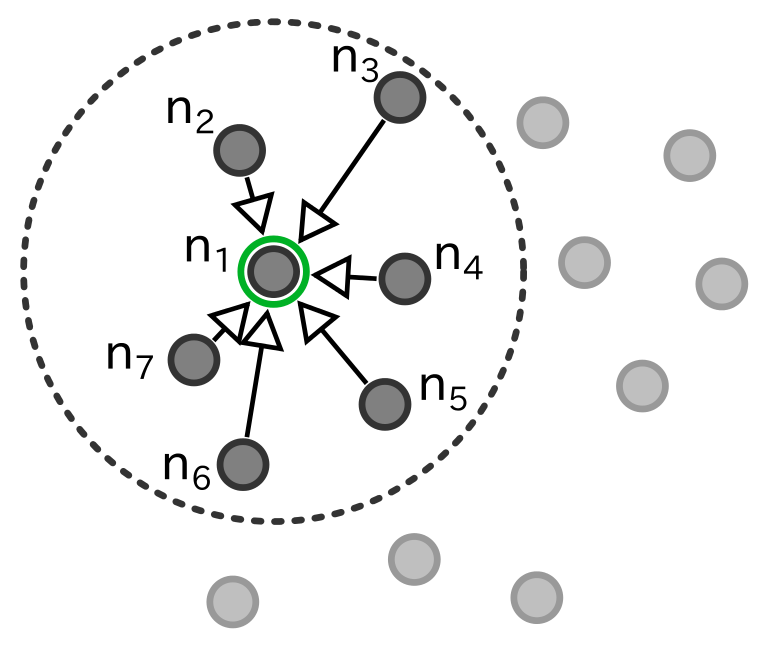
\includegraphics[scale=1.0]{figures/coordinator-4.png}
				\label{figure:Formation of fully meshed computation group - d}
			}\\
			\subfloat[]{%
				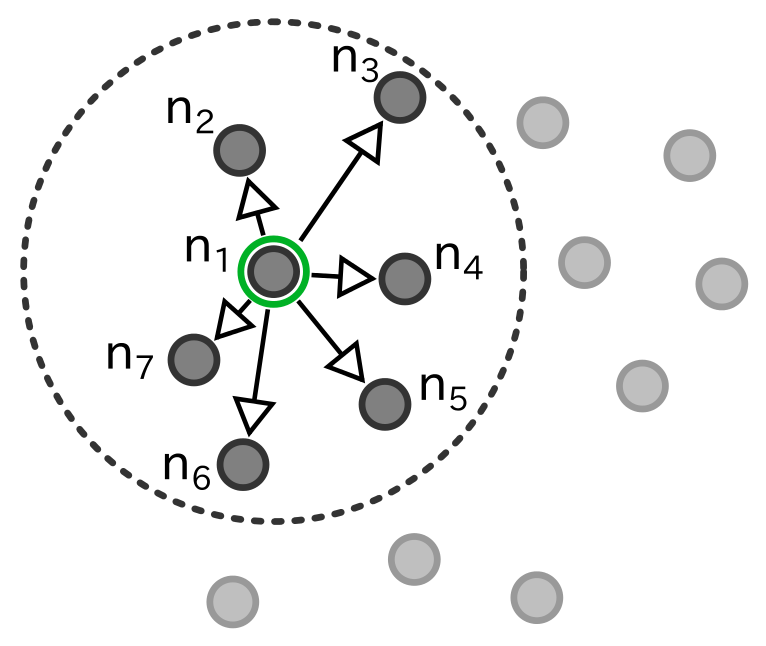
\includegraphics[scale=1.0]{figures/coordinator-5.png}
				\label{figure:Formation of fully meshed computation group - e}
			}%
			\hfill
			\subfloat[]{%
				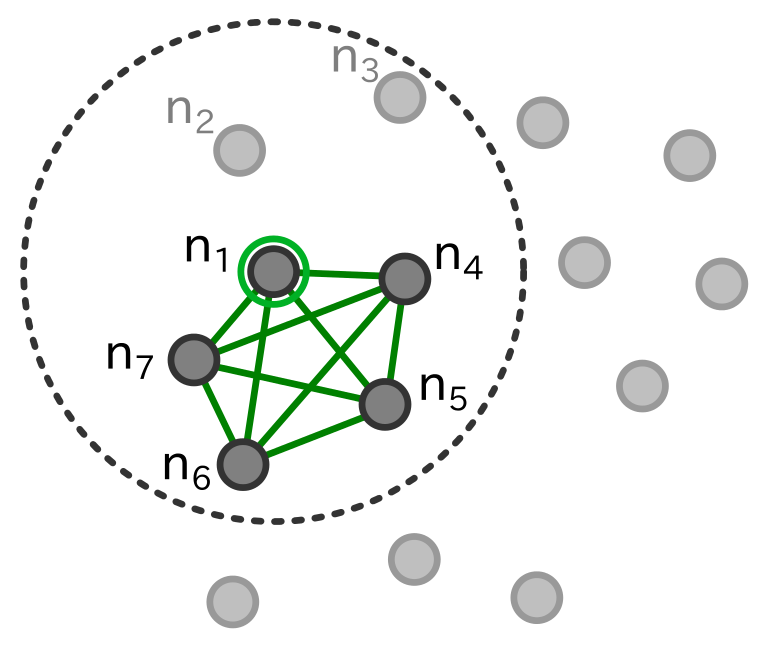
\includegraphics[scale=1.0]{figures/coordinator-6.png}
				\label{figure:Formation of fully meshed computation group - f}
			}
		\end{figure}
		
		Since parallel message exchange for the computation group cannot be guaranteed (see \ref{Implementability}), the coordinator controls sequential message exchanges with token passing in accordance with \ref{req:Token-Passing}. For example when $n$ nodes want to exchange $n$ secrets divided into $n$ shares each, the coordinator first requests successively the shares for himself ($s_i,1$) from the other $n-1$ nodes, while transmitting his own shares ($s_1,j$) with the request. Then the communication token gets passed to the next node, which in turn requests the shares for himself from the other $n-2$ nodes while transmitting his own shares and so on. An exemplary share-exchange for $n=3$ with token-passing is illustrated in figure \ref{figure:coordinator token passing}.
		
		\begin{figure}[!htb] % h for placement here
		\caption{\gls{UML} sequence diagram for passing of communication token} \label{figure:coordinator token passing}
		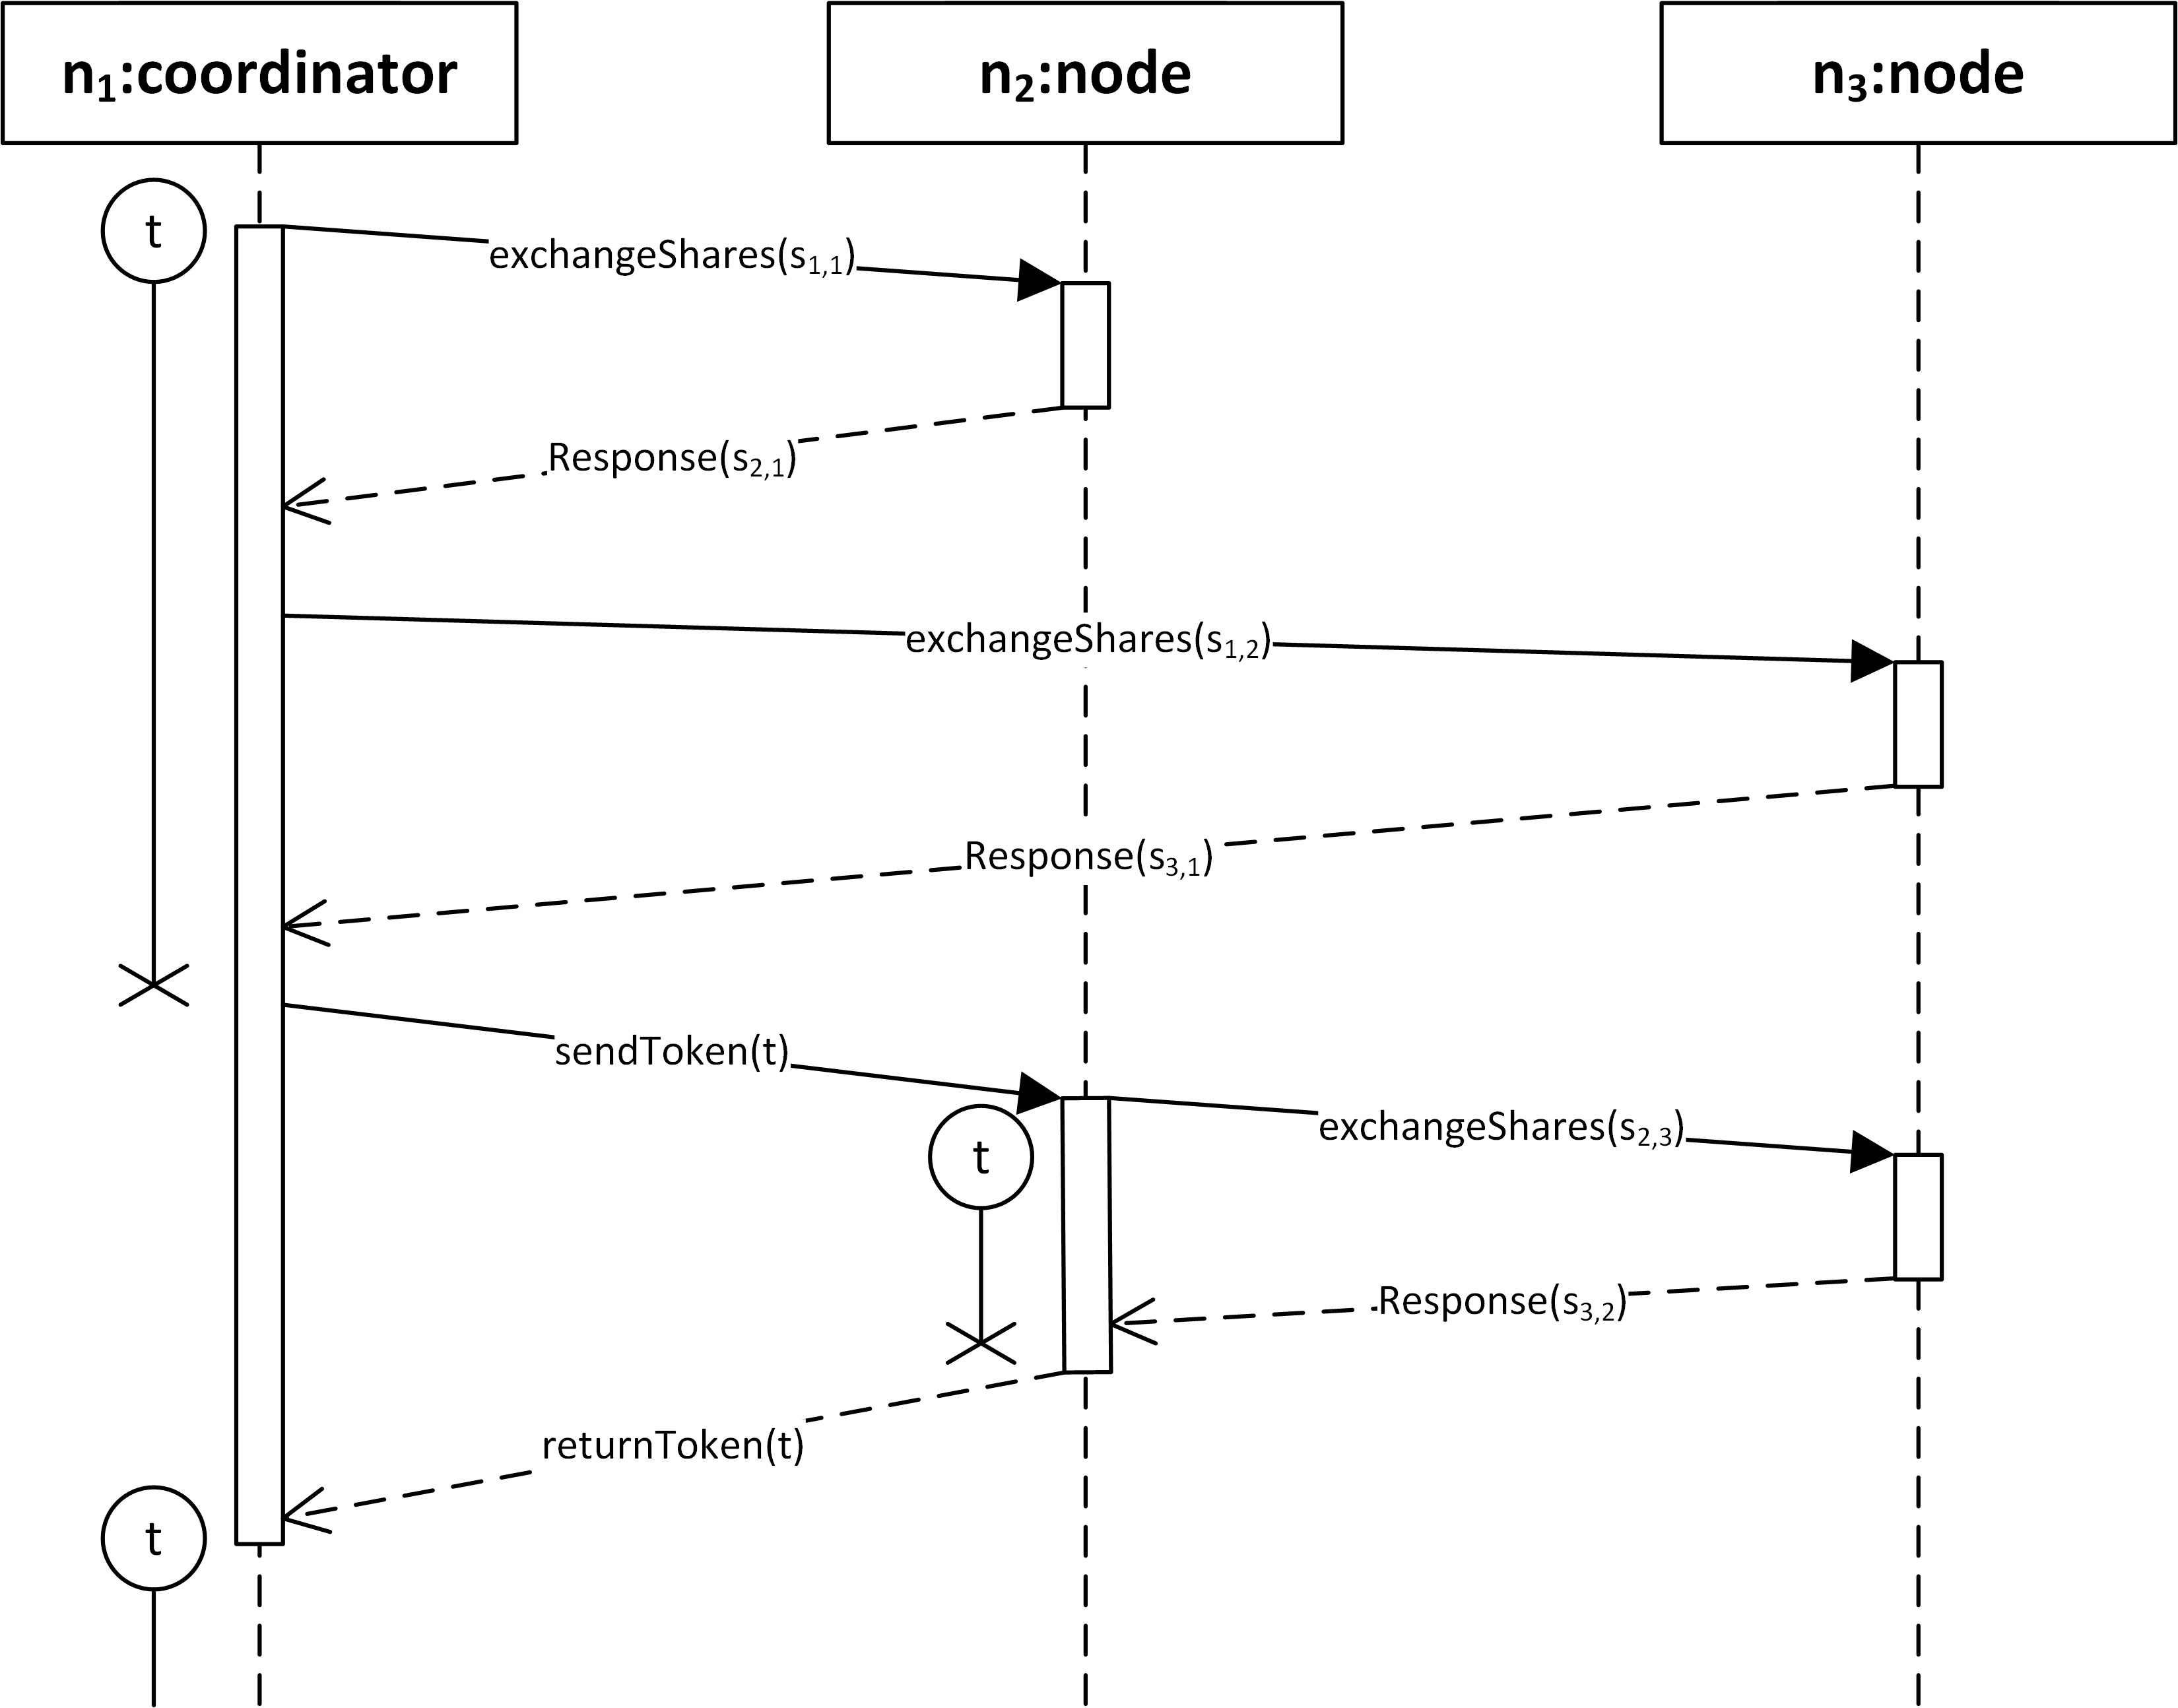
\includegraphics[scale=1.0]{figures/token-passing.png}
		\end{figure}
		
		The combination of processes with the same communication partners, single-digit bytes of payloads and short process termination is a good option to reduces the total message-occurrence in the network: for example when a coordinator requests the states of nearby nodes, it can be combined with the clock synchronization.
		
		\FloatBarrier
		
		\subsection{Clock Synchronization} \label{Clock synchronization}
		
		For statistical data in a gamification system, the sequence of events in infinitesimal time units is not as important as comparing the data for the same durations in \gls{UTC}, so a synchronization of physical clocks is needed as requested in \ref{req:Clock Synchronization}. In this thesis  the well known Berkeley-algorithm for internal clock synchronization in distributed systems is used as described in \textcite{Ghosh2015}.
		
		\noindent The coordinator
		%\vspace{-\topsep}
		\begin{enumerate}
			%\itemsep-0.5em
			\item requests the current time values $t_i$ from participating nearby nodes $i$.
			\item computes the average of these values $t_{average}$.
			\item reports back the adjustments $\Delta_{i}=t_{average}-t_i$
		\end{enumerate}
	
		Since the communication between the coordinator and a node takes time, the received response is already outdated. This is compensated by observing the \gls{RTT} and using half of the duration as a correction value (compare \ref{eq:berkeley RTT}). The \gls{RTT} is herein the timespan between sending a request to a node and receiving its response (see figure \ref{figure:berkeley RTT}).
		\begin{alignat}{1}
		t'_i &=t_i+\frac{RTT}{2}=t_i+\frac{t_e-t_s}{2} \label{eq:berkeley RTT}
		\end{alignat}
		
		\begin{figure}[!htbp] % h for placement here
			\caption{Round Trip Time} \label{figure:berkeley RTT}
			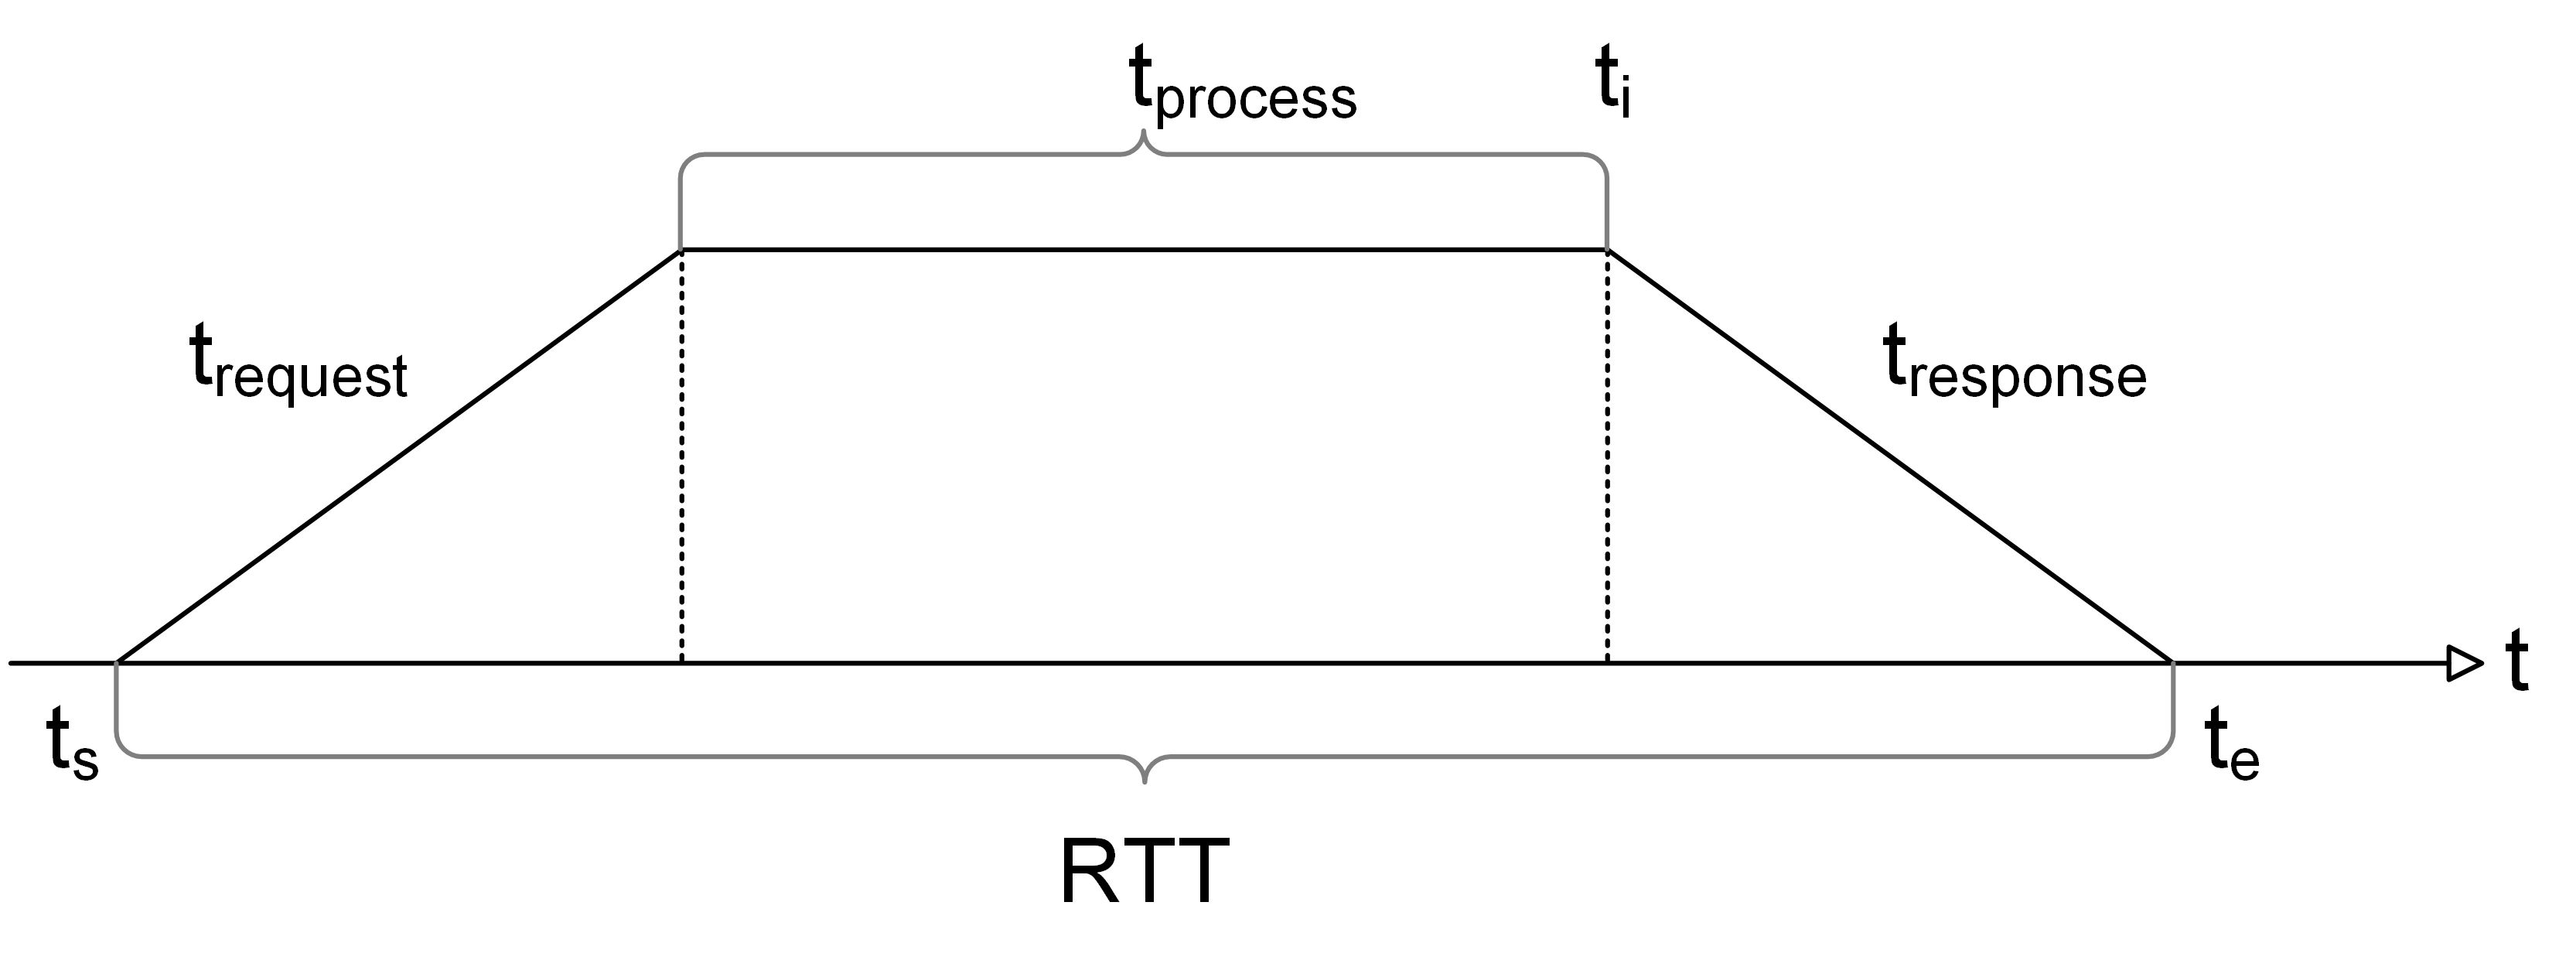
\includegraphics[scale=1.0]{figures/berkeley.png}
		\end{figure}
		
		 By sending the adjustments $\Delta_i$ instead of the adjusted time, the receiving nodes do not need to compensate the received value with the \gls{RTT}. Figure \ref{figure:berkeley example} depicts the computation of the adjustments using Berkeley with \gls{RTT} correction for three nodes. 
		
		\begin{figure}[!htbp] % h for placement here
			\caption{Example computation of adjustments with Berkeley} \label{figure:berkeley example}
			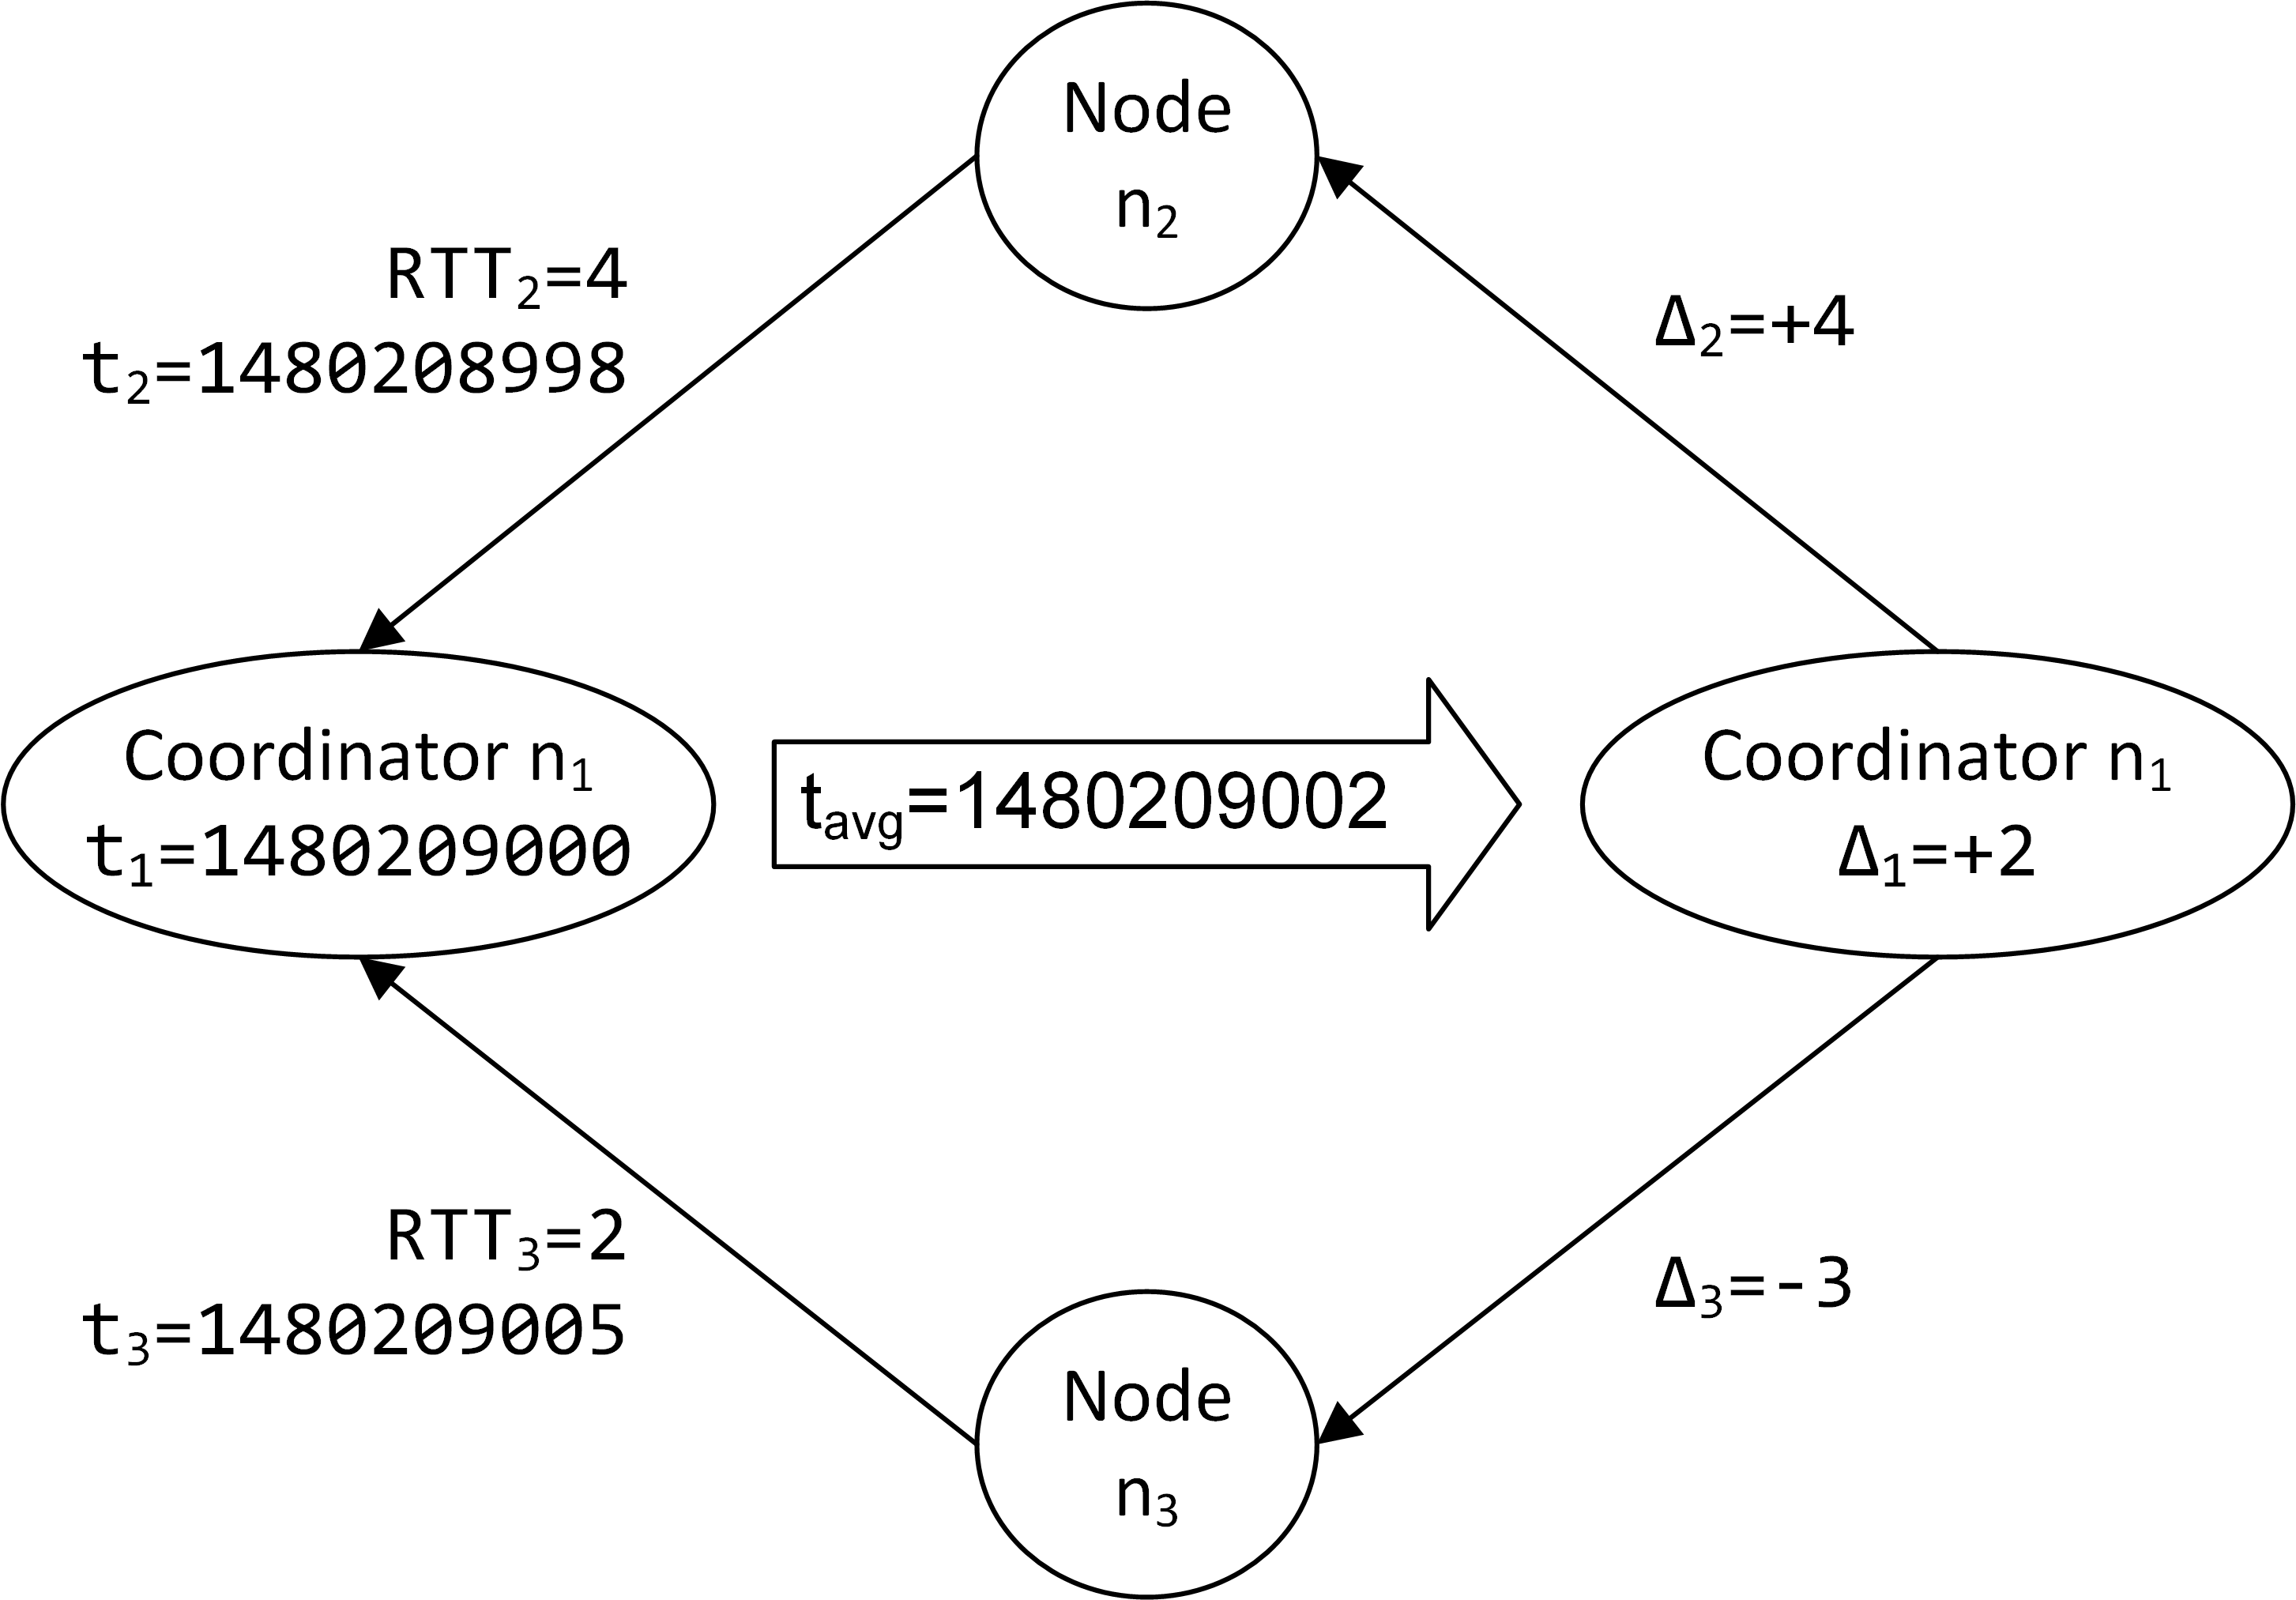
\includegraphics[scale=1.0]{figures/berkeley-example.png}
		\end{figure}
	
		 For further improvement of the accuracy the processing duration between receiving a request and sending the response $t_{process}$ can be measured and send to the coordinator. In this thesis the simple approximation for $t_{response}$ is used, since the additional payload extends the transmission duration. The \gls{RTT} has to be below an upper bound though, otherwise there is to much uncertainty regarding the influence of $t_{request}$, $t_{process}$ and $t_{response}$.
		 Also bounds for the deviation of the time can be defined to reduce the influence of outliers.
		 
		 The framework does not change the actual clock setting on the hosting system, but stores the computed time difference $\Delta_t$ and applies the value to all time-related actions. To make sure that a node is time-synchronized before scores and computations are acquired, it is reasonable to trigger a synchronization when the node joins the network. 
		 
		\FloatBarrier
		
		\subsection{Non-termination Detection} \label{Non-termination Detection}
		
		Especially since the coordinator gives temporarily away the message token and goes into a waiting state, there has to be a protocol to detect non-termination for processes. Meeting \ref{req:Non-termination Detection} each request to another node and each local computation initializes the start of timers. The local timer triggers the transmission of a heartbeat message (compare \ref{req:Heartbeat}) to the coordinator, signaling that the process is still intact, but not yet finished. If the coordinator receives a heartbeat message, it informs the other nodes in the computation group (causing them to reset their local timers), and resets its local timeout-timer. If the coordinator reaches a limit for the timer without receiving a heartbeat message, non-termination is assumed and all group members are informed, that the computation failed. The heartbeat protocol for the coordinator waiting for response is outlined in figure \ref{figure:heartbeat coordinator}, while the protocol for a node in possession of the message token is displayed in figure \ref{figure:heartbeat node}.  
		
		\begin{figure}[!htb] % h for placement here
			\caption{Avoidance of false non-termination detection through heartbeat messages} \label{figure:False non-termination detection with heartbeat messages}
			\centering
			\subfloat[]{%
				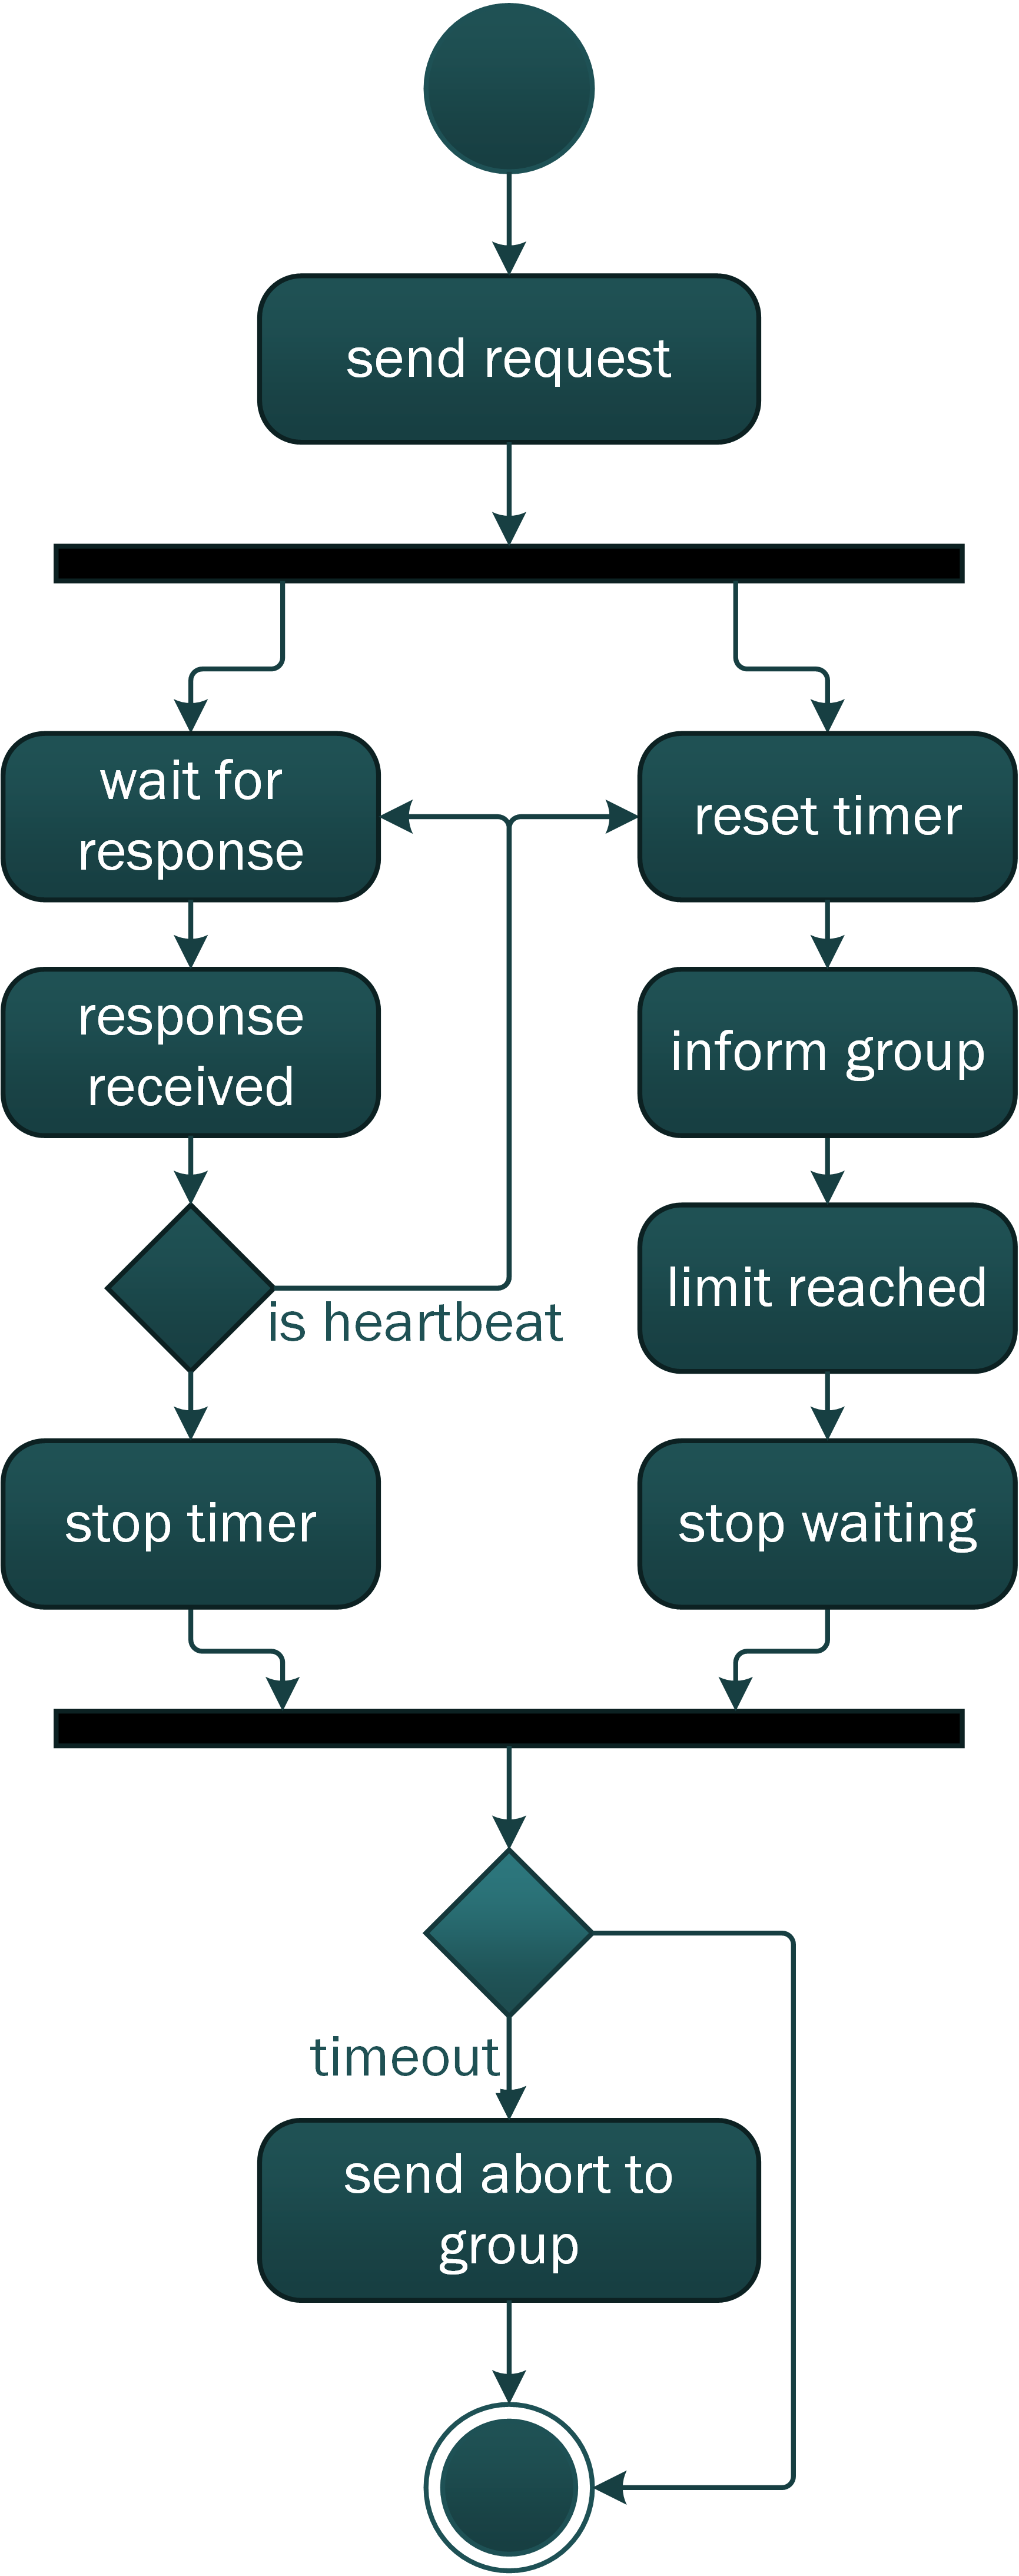
\includegraphics[scale=0.8]{figures/heartbeat-coordinator.png}
				\label{figure:heartbeat coordinator}
			}%
			\hfill
			\subfloat[]{%
				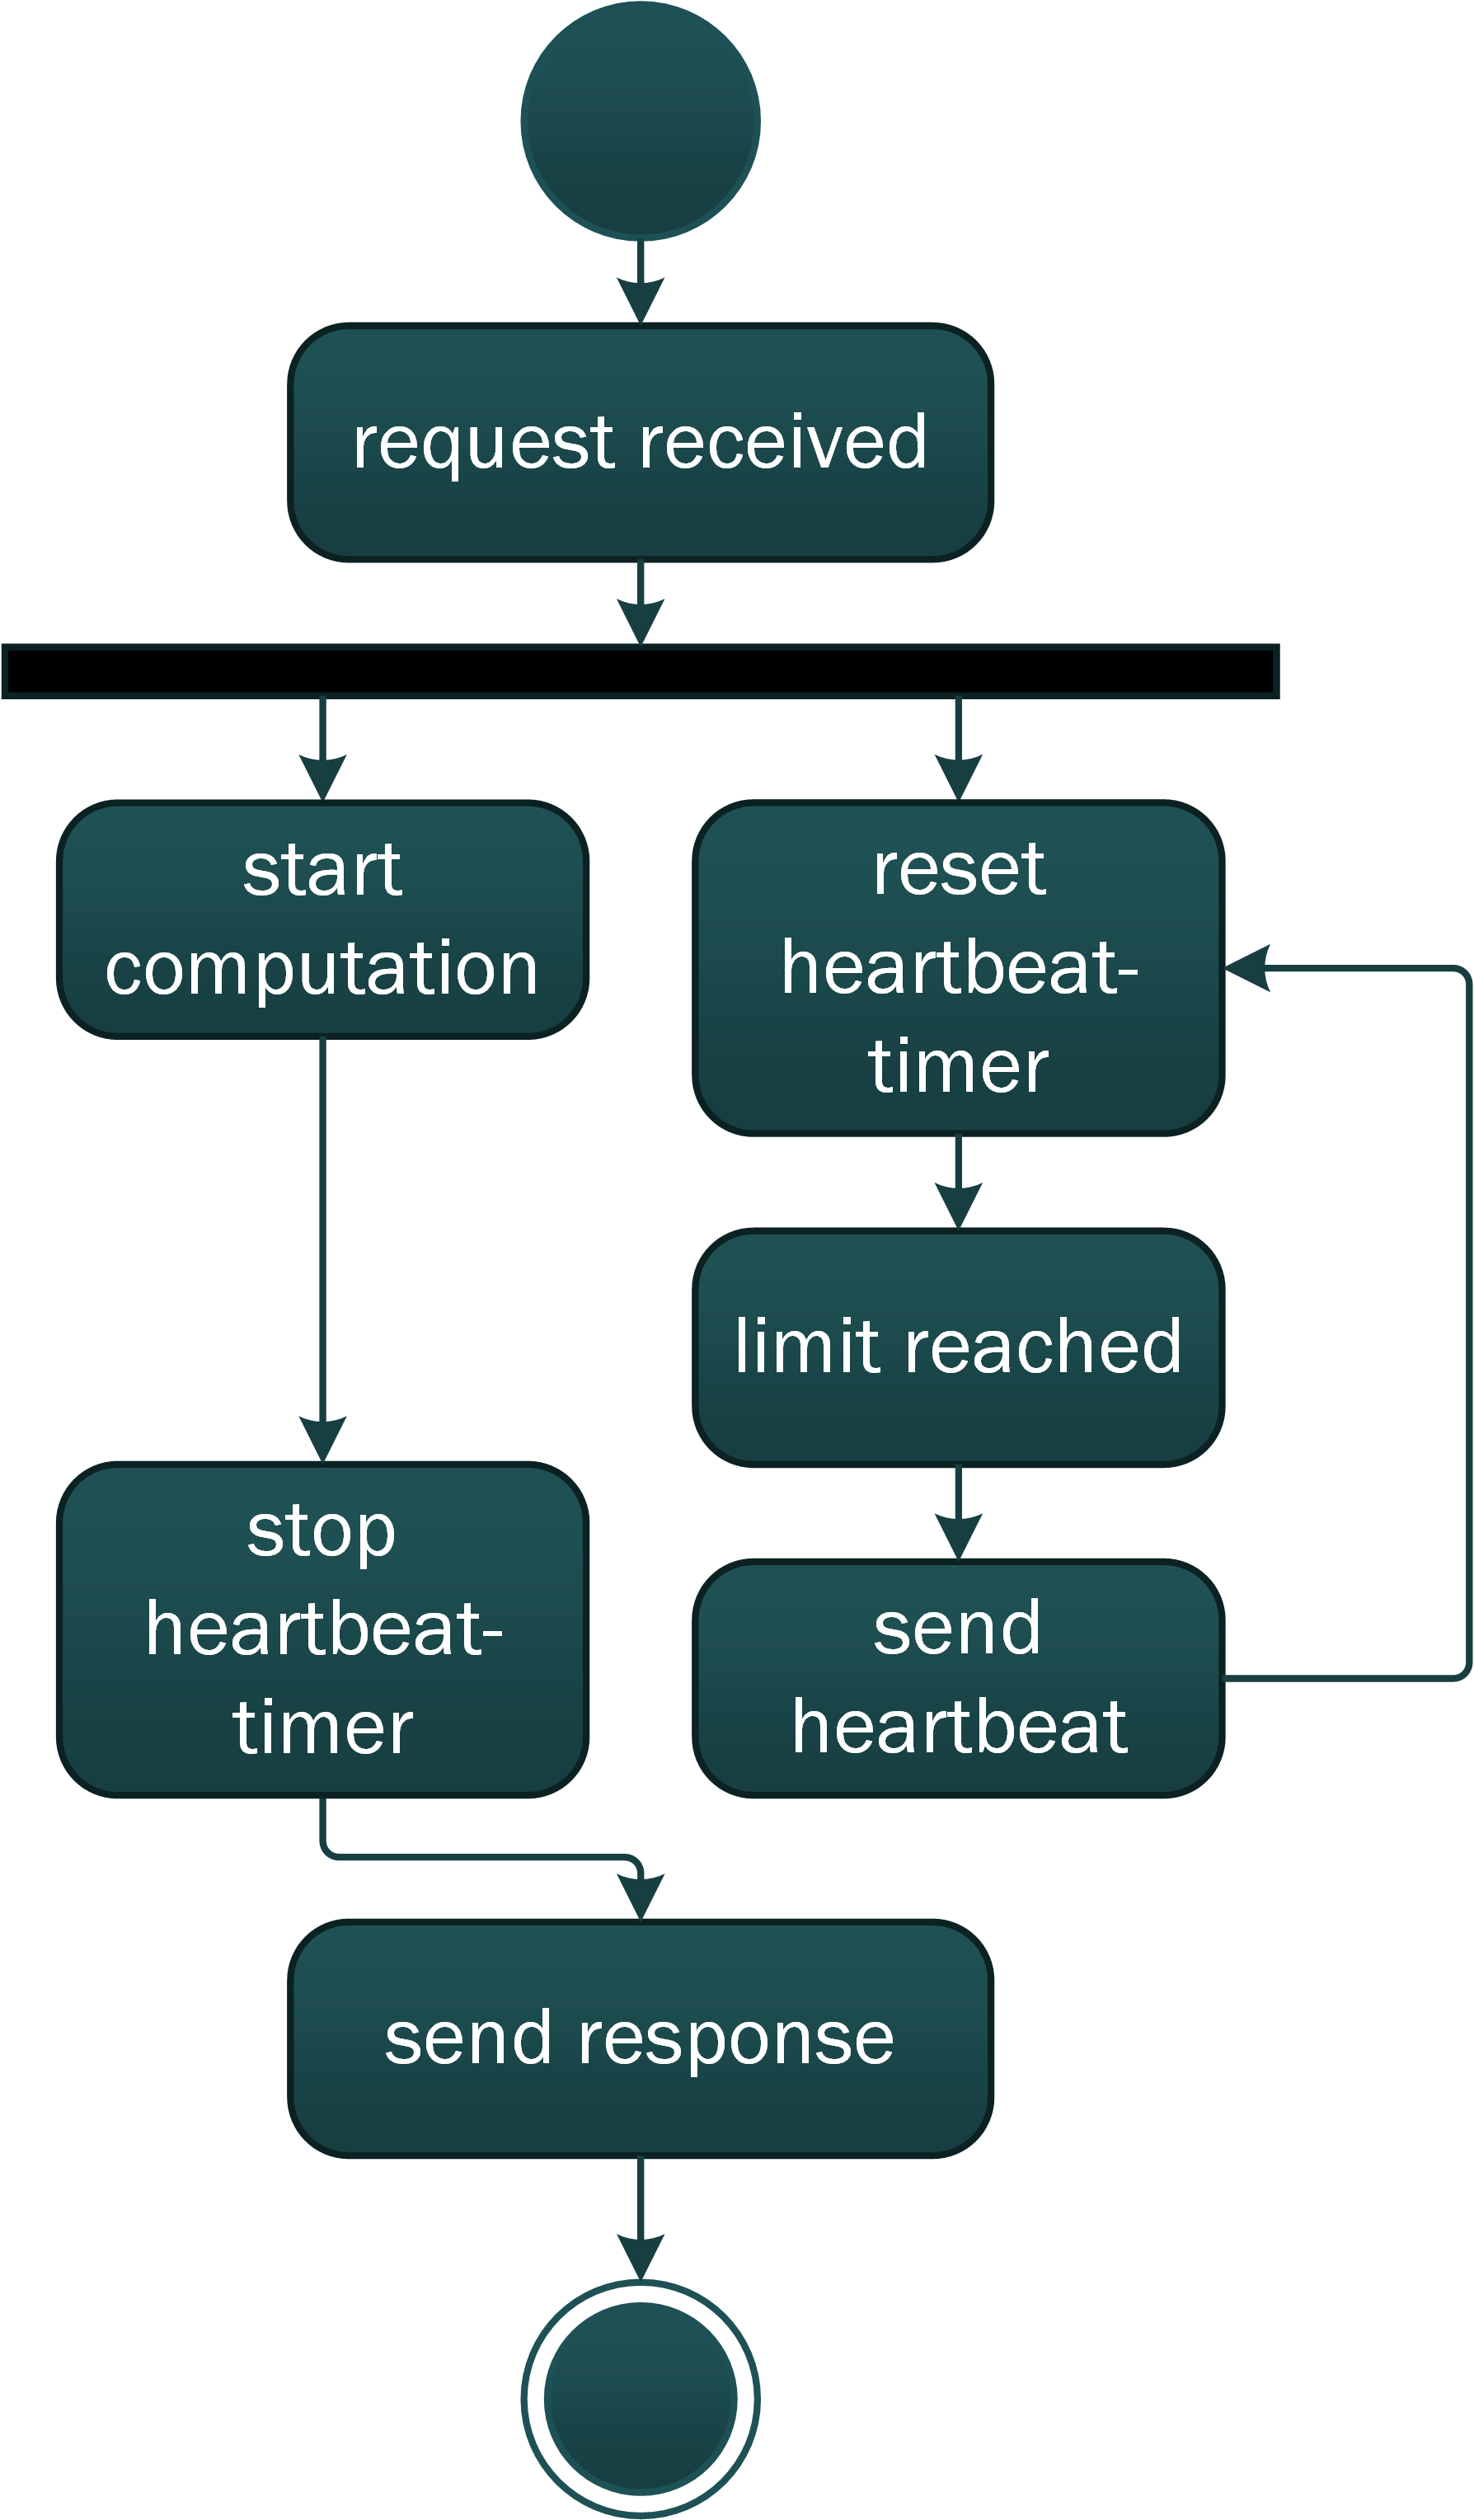
\includegraphics[scale=0.8]{figures/heartbeat-node.png}
				\label{figure:heartbeat node}
			}
		\end{figure}
		
		\FloatBarrier
		
		\subsection{Distributed Databases} \label{Distributed Database}
		
		A distributed system without central servers, that guarantee availability throughout the network, has to provide a distributed database model. This means, that nodes need to compare their database states with each other and synchronize differences. Since the nodes can enter and leave the network freely, preservation of the data in the system as well as consistency has to be considered.
		
		The framework deals only with entry-sets of the database and lets the hosting system handle the actual storage. Since each node hosts its own database, transactions for concurrent access is not an issue.
		
		\noindent An entry consists of:
		%\vspace{-\topsep}
		\begin{itemize}
			%\itemsep-0.5em
			\item Hash over the entry
			\item Unix timestamp
			\item size of computation group
			\item indicator for min, max or sum
			\item value
		\end{itemize}
		
		The combination of hash and Unix timestamp generates a key for the entry that is most likely collision free. The size of the computation group is needed to compute the arithmetic average from multiple entry-sum-values in a specified time-window: 
		\begin{align*}
			\begin{rcases*}
				\begin{rcases*}
					\mathmakebox[2.5cm][c]{ \underbrace{s_1, s_2, s_3, s_4, s_5}_{n_1=5} }  & \quad
				\end{rcases*} v_1=\sum_{i}s_i \\
				\begin{rcases*}
					\mathmakebox[2.5cm][c]{ \underbrace{s_6, s_7, s_8}_{n_2=3} } & \quad
				\end{rcases*} v_2=\sum_{i}s_i
			\end{rcases*} \overline{v}_i=\frac{v_1+v_2}{n_1+n_2}
		\end{align*}
		 
		Since the framework offers three types of \glspl{SMPC} the entry must reflect the source of the value. By comparison and updating, each node will have eventually all entries, so a distributed database has eventual consistency.
		To meet with the requirement \ref{req:Database Synchronization} each node holds the sum of the entries' hashes within a specified time-window. This value is used to compare the database-states between nodes: if the values are equal, the databases are likely consistent (collisions are possible though), otherwise entries are compared and exchanged. First the coordinator request the hash-sum. If they match an acknowledgment is send, otherwise up to n (predefined upper bound) hashes of the entries in anti-chronological order are send in an array to the node. The node response with an array of booleans, representing if the hashes are known. If the response-array contains zeros, then the unknown entries are transmitted. After an entry-exchange the hash-sums are compared, to determine if consistency is reached (coordinator request hash-sum if needed, compare figure \ref{figure:Database synchronization scheme}). If the hash-sums do not match, the node sends up to n entry-hashes to the coordinator, skipping already evaluated entries. This is repeated until consistency is reached or a request times out and the process is aborted.
		Figure \ref{figure:Database synchronization scheme} displays the basic process for $n=2$, with ASCII-values as hashes:
		
		\begin{figure}[!htbp] % h for placement here
			\caption{Database synchronization scheme} \label{figure:Database synchronization scheme}
			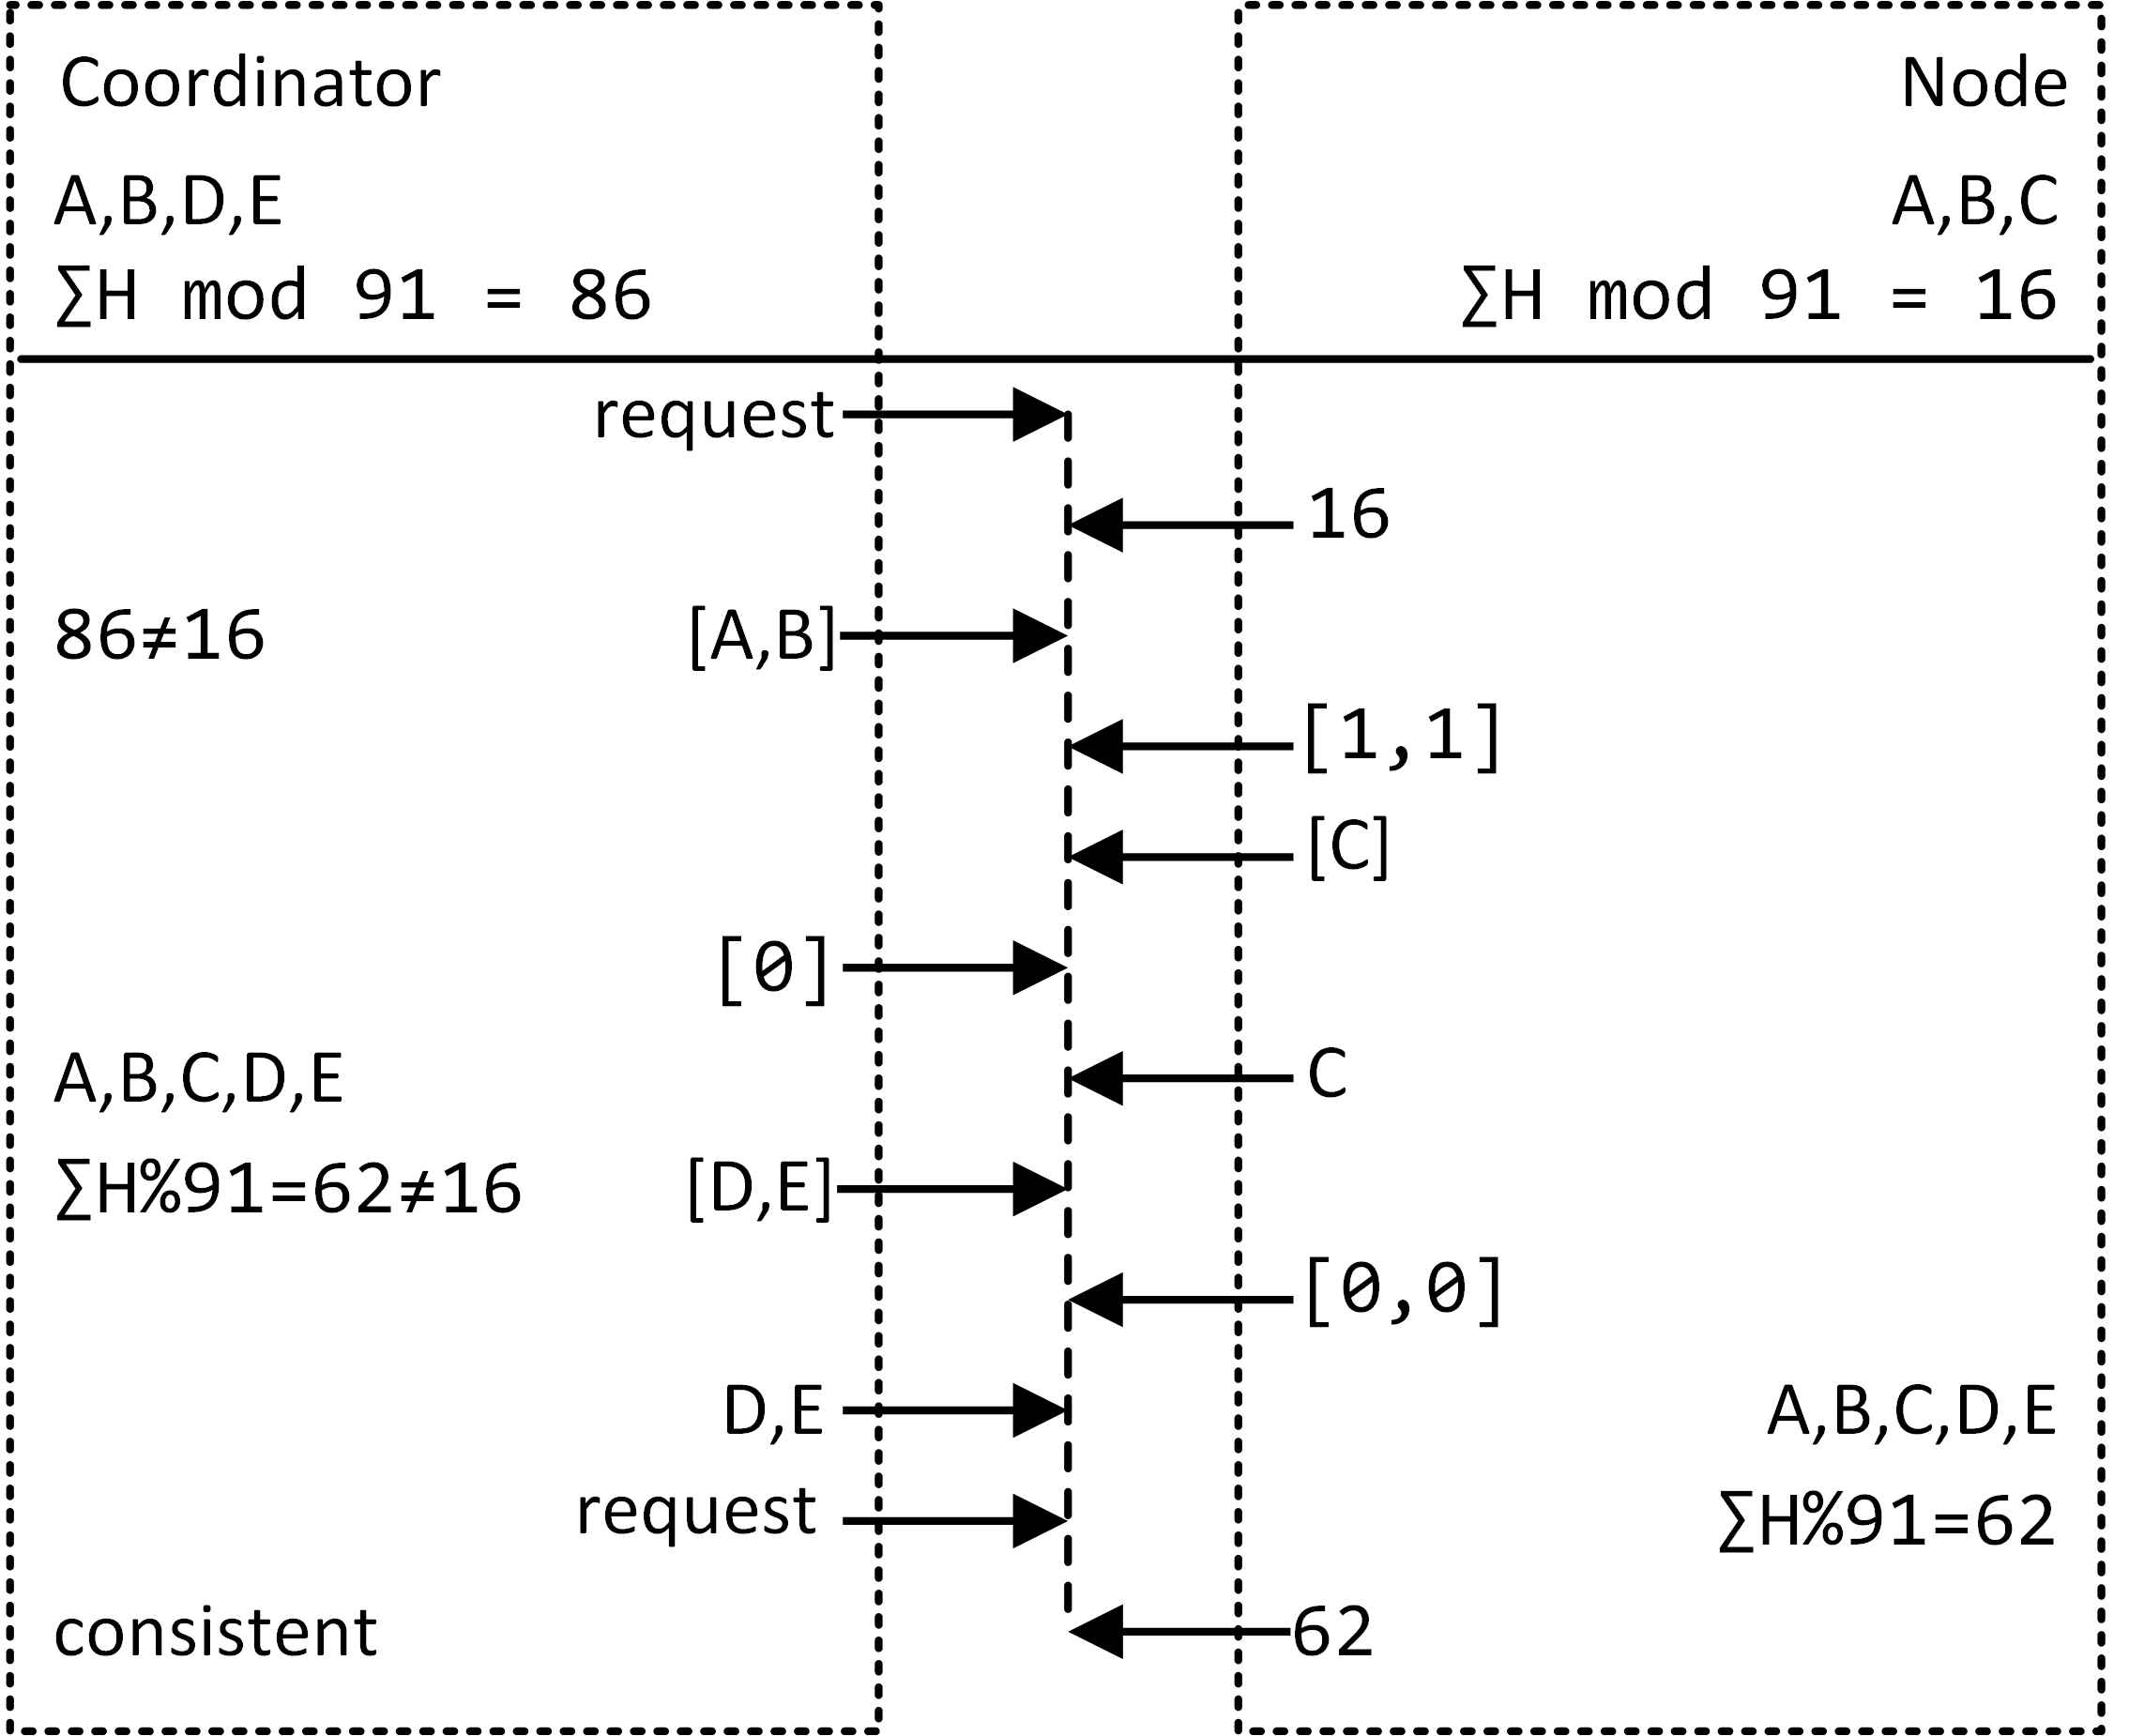
\includegraphics[scale=1.0]{figures/db-synchronization.png}
		\end{figure}
		
%	\section{Applicability of \gls{SMPC} Protocols in \gls{MANET}s} \todo*{Remove Applicability chapter? More or less answered in previous/following chapters...}
	
%		\subsection*{Analysis of Key Factors: Computing Power, Network Data Rates and Duration of Connection}
		
%		\subsection*{Effectiveness of \gls{SMPC} Protocols in Sparse Networks}
		
%			\subsubsection*{Maintaining anonymity}
		
%			\subsubsection*{Strategies for Aggregation of Participants in Sparse Networks}

	\FloatBarrier
	
	\subsection{Securing the Communication Channel} \label{Securing the Communication Channel}
	
	As requested in requirement \ref{req:SMPC Module} and noted in \ref{Secure Addition Protocol} the \gls{SMPC} protocols need secure communication channels. Listen in on wireless communication means receiving the radio signals, so for common wireless technologies this is easily accomplished. Since the physical layer is more or less public, the communication needs encryption. 
	For this framework two kinds of encryption are used: first asymmetric cryptography is used to exchange a session-key, which is then used to secure messages with symmetric encryption, as displayed in figure \ref{figure:RSA/AES scheme}. This principle is well known from \gls{TLS} encryption used in \gls{HTTPS}. For the symmetric encryption the \gls{AES} as described by \textcite[pp. 19-25]{Delfs2015} is used.
	For the asymmetric encryption the public-key cryptosystem \acs{RSA} as described by \textcite[pp. 49-76]{Delfs2015} is used.
	\gls{AES} encrypts and decrypts faster than \gls{RSA}, because \gls{RSA} requires long keys (2048 bit and longer recommended) for proper security. But \gls{AES} needs sender and receiver to know the cipher, and the exchange of this key over an insecure channel only with \gls{AES} is not possible.
	
	\begin{figure}[!htbp] % h for placement here
		\caption{Securing communication with \gls{RSA} and \gls{AES}} \label{figure:RSA/AES scheme}
		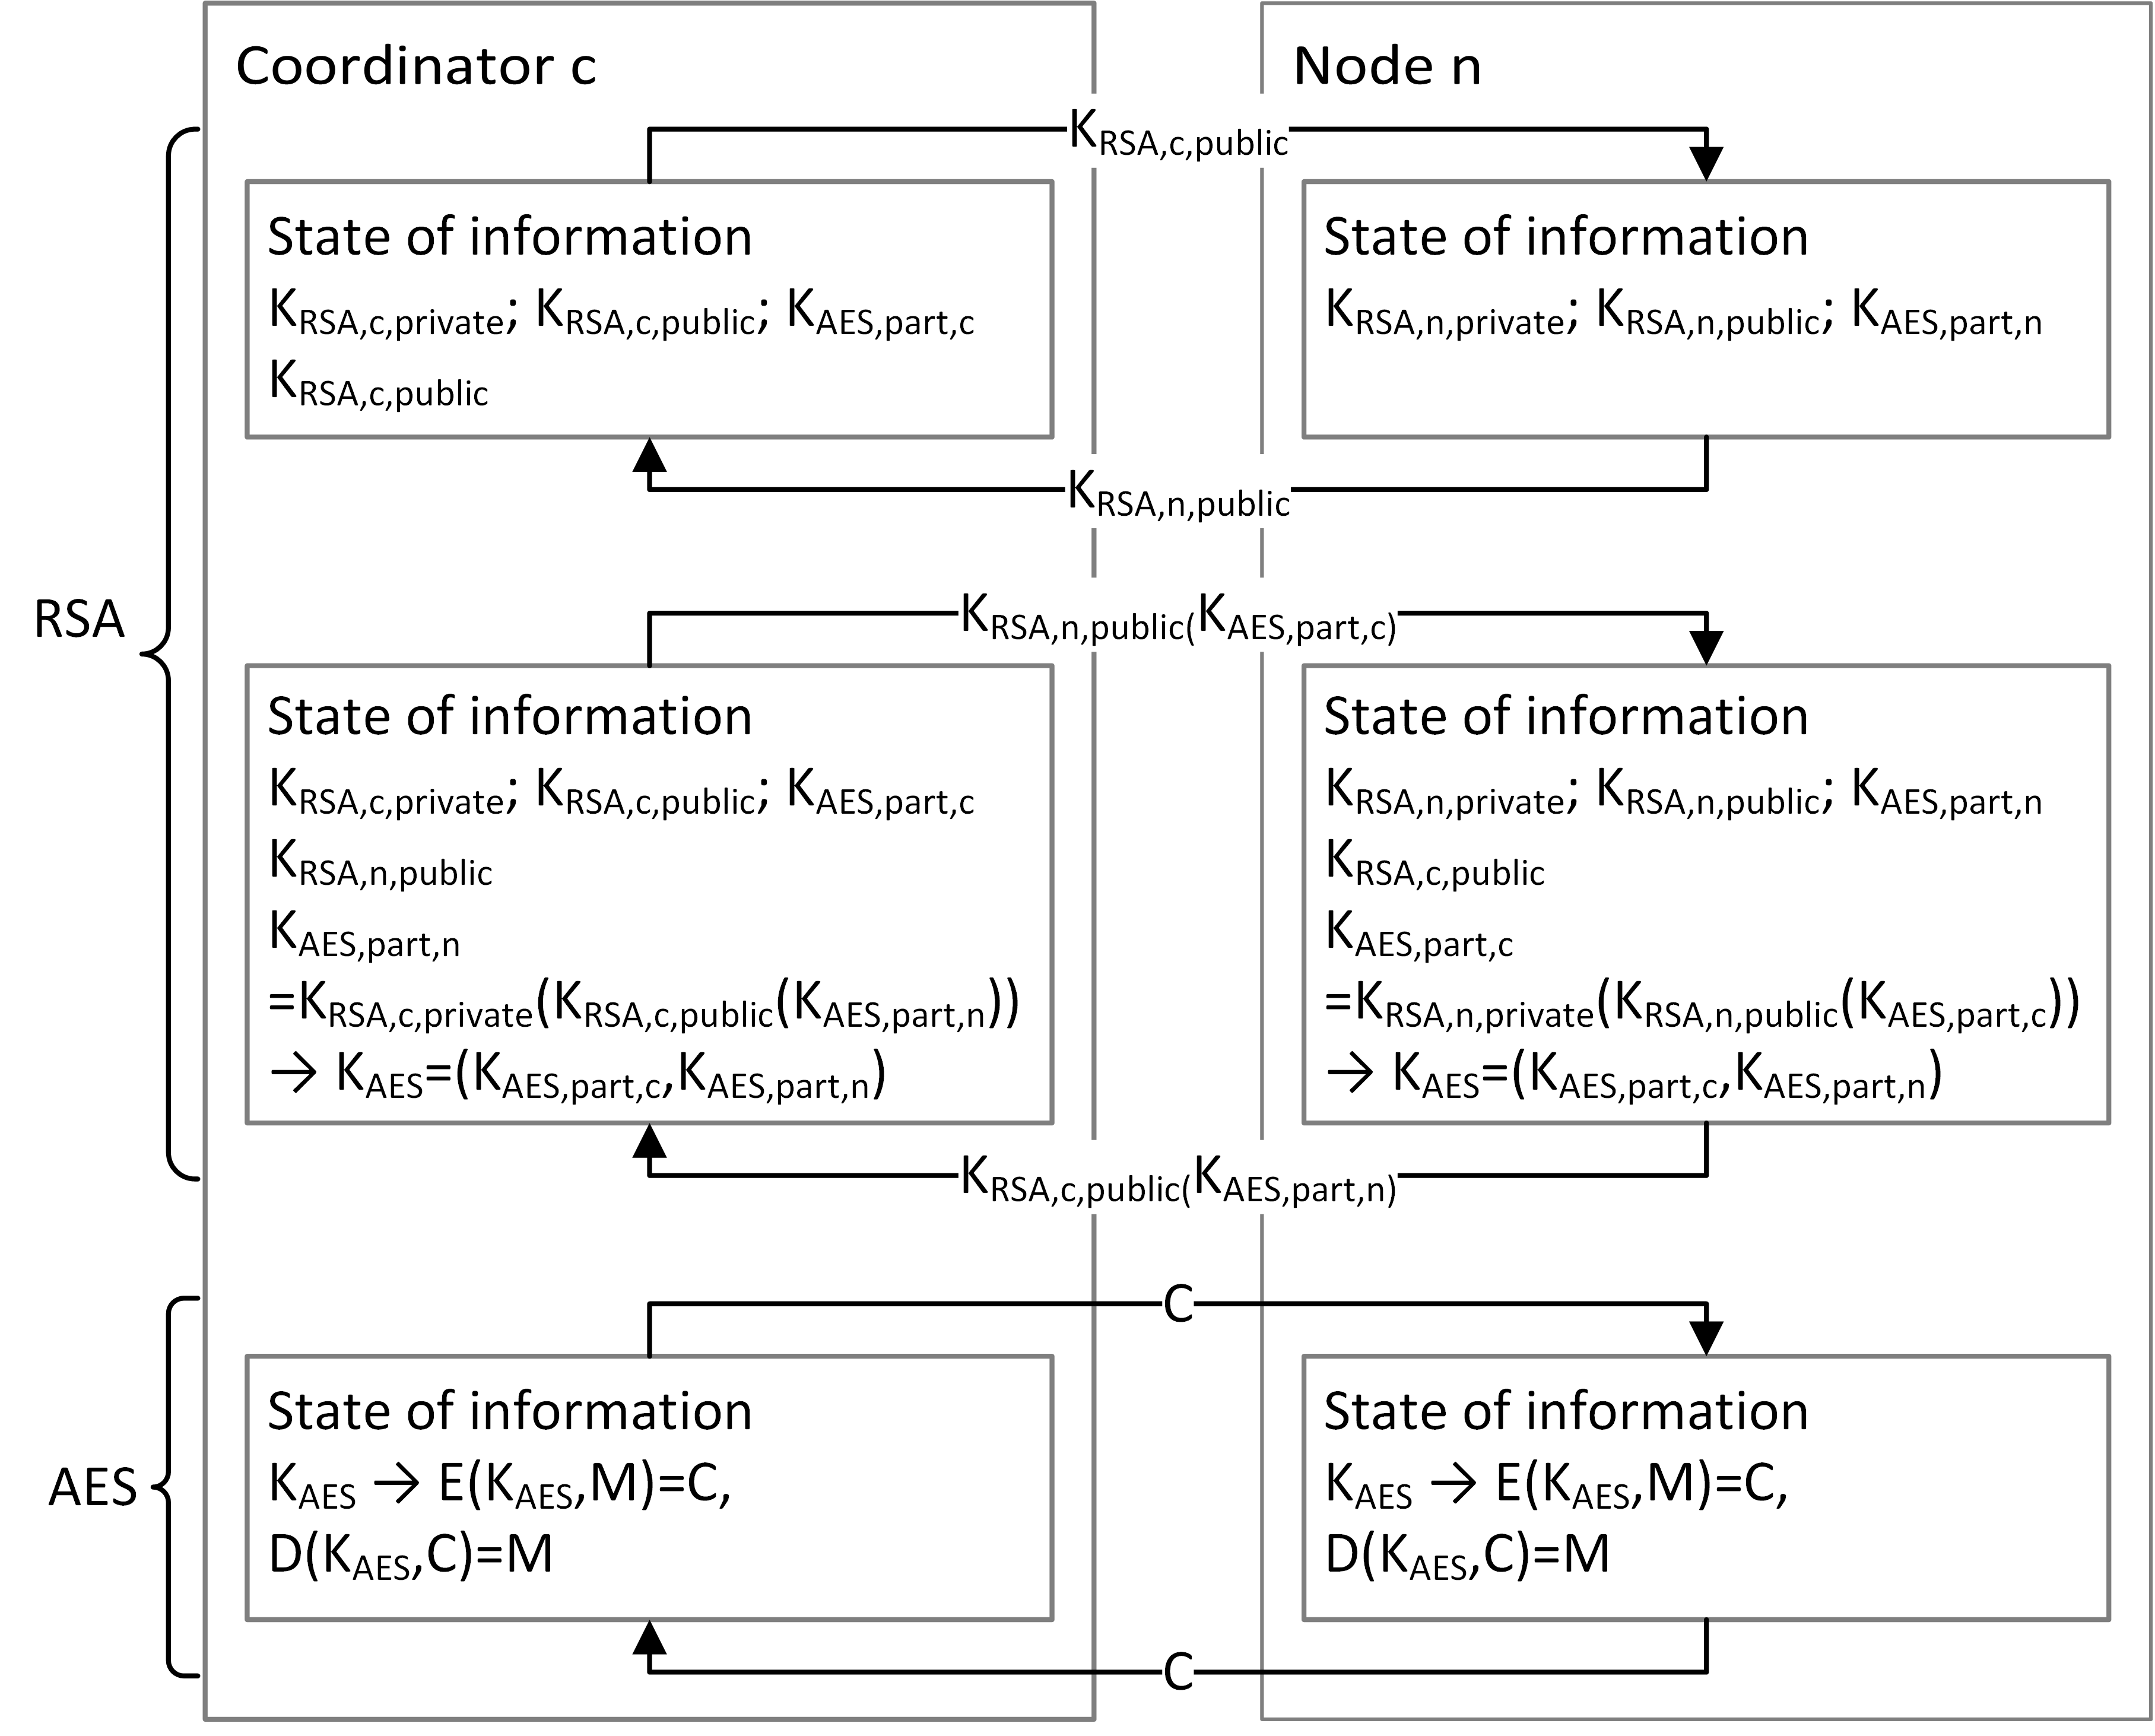
\includegraphics[scale=1.0]{figures/encryption.png}
	\end{figure}
		
	The basis for the cryptosystem by \gls{RSA} is the prime-factorization, which requires super-polynomial time. \gls{RSA} is asymmetric, since there is one key for encryption and one key for decryption. In this setting, the public key is used for encryption, so only the receiver with the private key can decrypt the secret.
	For the key generation two large prime numbers are selected: $p,q,p\neq q \in \mathbb{P}$. The product $n=p\cdot q$ is computed. Euler's Phi function $\phi (n)=(p-1)(q-1)$ is computed and a coprime integer $e$ is selected $1<e<\phi(n)$. A common value for $e$ is $65537$. $n$ and $e$ form the public key.
	The private key is formed from $n$ and $d$, where d meets $e\cdot d\equiv 1\mod \phi(n)$.
	For the symmetric encryption, booth partners use the same key. \gls{AES} is an iterated block cipher with a block length of 128 bits and key length of 128, 192 or 256 bits. The iterations (called rounds) follow the Rijndael algorithm. A detailed description of the algorithm can be found in \textcite[pp. 20-25]{Delfs2015}.
	
	\FloatBarrier
	
	\section{Architecture} \label{Architecture}
	
	Based on \ref{Coordinator Election} it is sensible, that the central element in this framework is a node component. Figure \ref{figure:UML component diagram} displays the \gls{UML} component diagram for the framework design and illustrates the basic conjunctions between the components, as well as key-functionalities. The node component can also act as the coordinator and in either state communications and computations let it pass through different states of activity. This framework therefor uses the state pattern: the current state determines the behavior and abilities of the node.
	In regard to the hosting system the node component utilizes a \gls{API} component, which uses callbacks to bind the communication layer and the system clock to the framework in accordance with \ref{req:Supportability}. To handle the message encryption a cryptography module is needed, providing the functionality described in \ref{Securing the Communication Channel}. As described in \ref{Non-termination Detection} a handler for timeout detection and heartbeat message triggering is provided. Parameters for communication, cryptography and \gls{SMPC} need to be accessible in a central component to meet \ref{req:Usability}.
		
	\begin{figure}[!htbp] % h for placement here
		\caption{\gls{UML} component diagram} \label{figure:UML component diagram}
		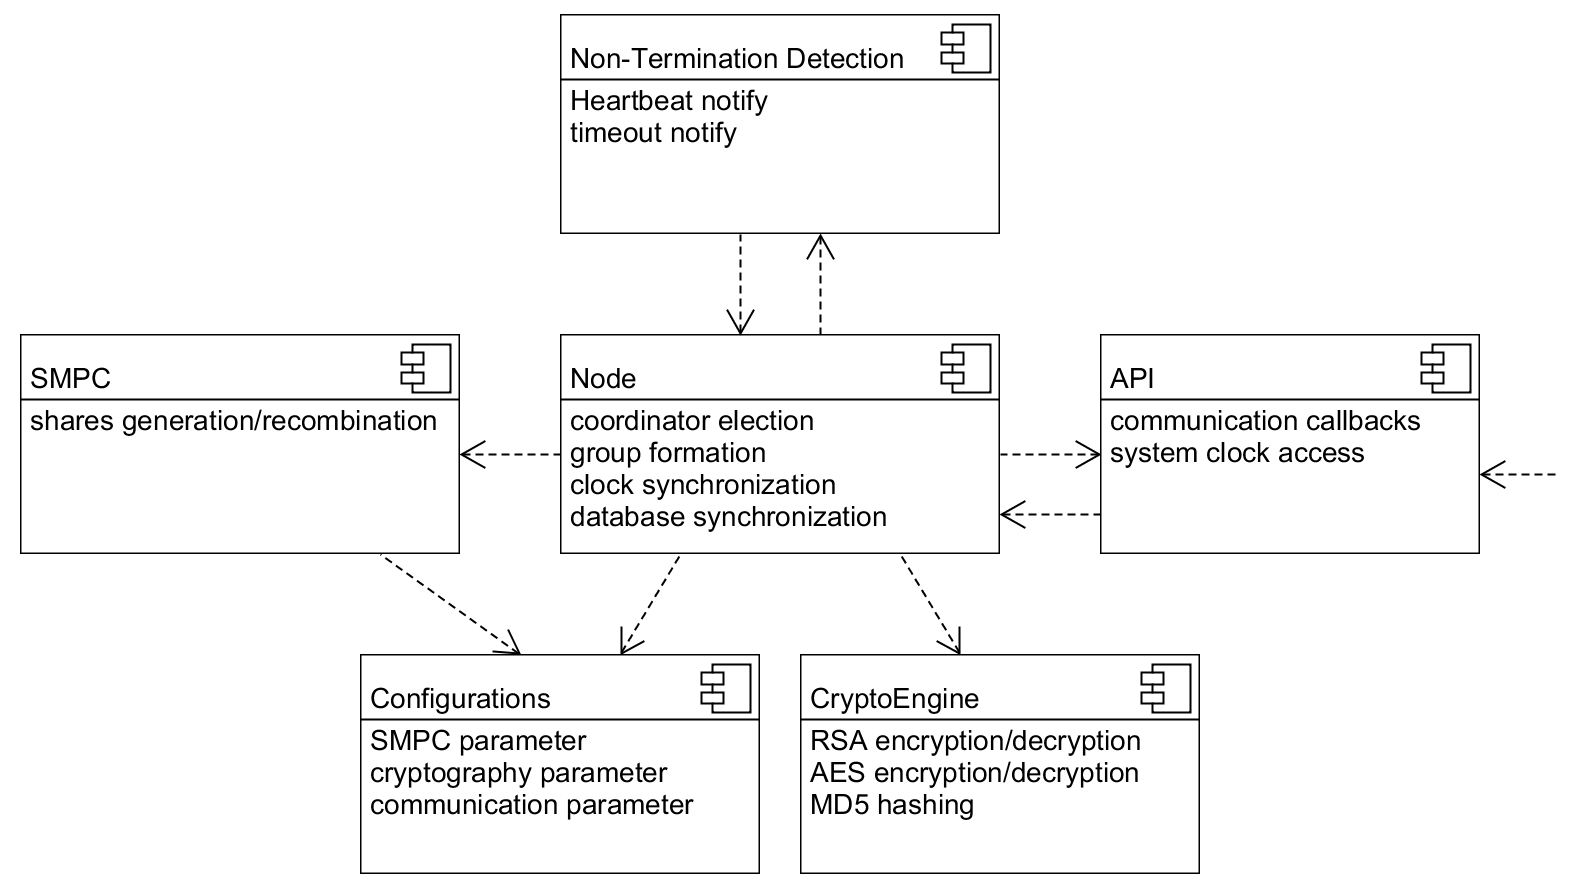
\includegraphics[scale=1.0]{figures/uml-component.png}
	\end{figure}
		
	Since it is likely, that the technical limitations described in \ref{Implementability} will be overcome in future releases, the framework's core functionality is independent from the efforts to provide the self-forming network abilities (avoidance of code smell change preventer/shotgun surgery). So in case of full \gls{MANET} implementation only the node component has to be adopted.
	
	\todo*{state machine; state pattern; client server architecture; \gls{UML} state diagrams for 1. joining network (get time; set clock delta), 2. finding computation partners, 3. running computation, 4. compare database}

\FloatBarrier